% !Mode:: "TeX:UTF-8:Hard"
\ifx \allfiles \undefined
\documentclass[a4paper,12pt,twoside]{book}
%\usepackage{CJKutf8}
\usepackage[T1]{fontenc}
\usepackage{pifont}
\usepackage{graphicx}
\usepackage{capt-of}
\usepackage{color}
\newcommand{\linuxcommand}[1]{\texttt{\textcolor{blue}{\$ #1 \Pisymbol{psy}{191}}}}
\newcommand{\op}[1]{\textcolor{blue}{-#1}}
\newcommand{\hotkey}[1]{\framebox{#1}}
\newenvironment{screen}{\sffamily}{\rmfamily}

\usepackage{listings}
\definecolor{mygray}{rgb}{0.9,0.9,0.9}
\lstset{backgroundcolor=\color{mygray}, basicstyle=\small}
\lstset{morecomment=[s][\color{red}]{/*-}{*/}}
\newcommand{\Hilight}[1]{\makebox[0pt][l]{\color{yellow}\rule[-3pt]{#1em}{11pt}}}
\newcommand{\HilightLine}[2][yellow]{\makebox[0pt][l]{\color{#1}\rule[-4pt]{#2em}{13.9pt}}}


\begin{document}
%\begin{CJK*}{UTF8}{song}
\title{basic knowledge}
\author{yan zhao}
\date{}\maketitle

\else
\chapter{Developing Knowledge and Tool}
\fi

\chapter{Linuxl}
\section{Linux basic}
\begin{itemize}
		\item Ubuntu is for desktop, and Mint is sleek and quick, CentOS is for server, It's stable. \textbf{If you use virtual machine, recommend Mint, if you want to install linux directly on a computer, you can use Ubuntu system.}

\item There are two Interface Framework, Qt and GTK\@.  KDE is based on QT, and Gnome and Cinnamon(Mint) is based on GTK.  

\item You can use \linuxcommand{uname} to check basic information about your computer, detail can be seen uname --help. 
\end{itemize}
\subsection{Terminal tips}

 \begin{itemize}
  \item Move shortcut keys are list below:Ctrl+p can go to the previous command, this is very useful. 
\begin{center}
  \begin{tabular}{c|c}
 \hline shortcut & fucntion \\
\hline Ctrl+f,b & forward, backward character \\
\hline Ctrl+a,e & move start,end \\
\hline alt+f,b & forward, backward word \\
\hline Ctrl+p,n & previous, next line \\
\hline Ctrl+r & search command history \\
 \hline
  \end{tabular}
\end{center}

\item delete shortcut keys: You can use "hw" to delete previous character or word. "dd" use to delete forward character or word, "uk" to sentence begining and end. In Vim, the keyboard shortcut is not the same. 
\begin{center}
  \begin{tabular}{|c|c|}
 \hline shortcut & fucntion \\
 \hline Ctrl+l & clear the screen \\	
\hline Ctrl+u & delete forward to begin\\
\hline ctrl+k & delete backward to end \\
\hline Ctrl+w & delete backward word\\
\hline alt+d & delete forward word \\
\hline Ctrl+d & delete forward a character  \\
\hline Ctrl+h & delete backward a character  \\
 \hline
  \end{tabular}
\end{center}

\item bind -p will list all the shortcut
\item  About keyboard shortcut, I have good idea, that is to use left Ctrl and Alt together, because you can use your thumb to press Alt and use palm to
	press Ctrl\_L,(Even in my three laptops, I also can press Ctrl\_L easily by palm).
	So a shortcut can be defined below:
	\[ \left\{ \begin{array}{cl}
	            \textrm{move} & \left\{ \begin{array}{c} \textrm{other: Ctrl\_L} \\ \textrm{emacs: Alt\_L} \end{array}  \right. \\
		    \textrm{select} & \left\{ \begin{array}{c} \textrm{other: Ctrl\_L+Shift\_L} \\ \textrm{emacs: Alt\_L+Shift\_L} \end{array}  \right. \\
	           \end{array} \right. + \left\{ \begin{array}{c}
						\textrm{left character: J} \\
						\textrm{right character: L}\\
						\textrm{upward: I}\\
						\textrm{downward: k}\\
						\textrm{left word: U}\\
						\textrm{right word: O} \\
						\textrm{begin line: H}\\
						\textrm{end line: ;}\\
						\end{array} \right.
	\]
	Delete command is below: \\
	\[ \textrm{delete} \left\{ \begin{array}{l}
	            \textrm{left character: Backspace}  \\
		    \textrm{right charcter: Ctrl\_L+N} \\
		     \textrm{left word: Ctrl\_L+Backspace}  \\
		    \textrm{right word: Ctrl\_L+M} \\
		     \textrm{line: Ctrl\_L+P}  \\
	           \end{array} \right.
	\]
	

	Question 1: why always left Ctrl?  \\
	Answer: Now, if you are smart enough, you can found that there is rules inside. All the commands is left Ctrl add right hand character, becuase left Ctrl can be
	pressed by left palm and right hand is more flexible than left hand when you click the different character. \\

	Question 2: why other use Ctrl and Emacs use Alt. \\
	Answer: In common applications, Alt has been assign to trigger menu item, such as Alt+F will trigger File menu, so, I must use Ctrl. In Emacs, on the contrary,
	Ctrl has been used to trigger some common commands, so I use Alt key( and Alt is used not often as Ctrl).\\

	Question 3: How can I export my custom shortcut to other computers \\
	Answer: There are two kind of shortcut one is kate and other is kile, they store in \verb=.kde/share/apps/katepart/katepartui.rc= and \linebreak[4] \verb=.kde/share/apps/kile/kileui.rc=
	you can copy them and cover them in your computer. If version is different, Maybe it's a little difficult. But you can just do it within the application, it don't need very long time. \\
        \\
	By now, these customized shortcuts haven't been used in practical use. Anyway, you can use arrowkey, it don't need too much memory. But it is a good suggestion. You can learn how to define a customized shortcut. If you need to do a lot texting job, they are very useful.
	 %目前,这些键盘的定义我还没有在实践中使用过。毕竟,用箭头键太直接了,而按住ctrl在一些笔记本上不是太方便。 不过,他们依旧是一个很好的建议,以后当你使用大键盘,或者是比较密集的进行编辑工作的时候,还是非常值得尝试一下的。
  \item Ctrl+Alt+F1\ldots F6 switch terminal. Ctrl+Alt+F7 return back to GUI\@. When F7 doesn't work, you can try F8. 
\end{itemize}

\subsection{time}
\begin{itemize}
\item For linux file time: there are three time stamp: atime (access time), it is when the file was last read.\  ctime is the inode change time, while mtime is the file modification time.\  mtime changes when you write to the file. It is the age of the data in the file. \textbf{Whenever mtime changes, so does ctime, except you use touch command} But ctime changes a few extra times. For example, it will change if you change the owner or the permissions on the file.  

\item  timestamp will be used in many linux commands, ls -l will show modification time. and you can use \linuxcommand{stat fileName} to see all the three time. The can be used in find command. 

\item \linuxcommand{touch} can change time of a file or you can use it to produce an
            empty file.
            \linuxcommand{touch -a existFile} change access time and ctime. \linuxcommand{touch -t existFile} change modify time and ctime.   \linuxcommand{touch -c existFile} change a,c and m time. 
            
\item \linuxcommand{touch -t YYMMDDHHmm} will set mtime and atime to the date you want and it sets ctime to \textbf{NOW}. You have complete control over mtime, but the system stays in control of ctime. So mtime is a little bit like the date on a letter while ctime is like the postmark on the envelope. System use ctime to do backup job. An example can be found in my evernote book mark. 


\end{itemize}



\section{File and Dir}
\subsection{basic}
\begin{itemize}
\item A hard link points to the file by \textbf{inode}.  A symbolic link points to the file by \textbf{filename}. 
 
\item  There is no "real" hard link name; All hard links are equally valid names for the file. You can use \linuxcommand{ls -l}. The first number after the file mode is the link count(this count is represent hard link number).  For symbolic link, It just point to a filename, If origin file name changed, symbolic link will not be valid.   symbolic is very flexible,  It can be linked to a dir or It can be linked to different file system. but hard link has many restriction. 

\item \linuxcommand{find -L / -samefile path/to/foo.txt}find all files links to foo.txt

\item Absolute directory must begin with root directory /
    \item *.so is shared dynamic library in linux *.a is lib file.  *.sh is script file. *.tar or
        *.tar.gz *.tgz are compressed file.

     \item \textbf{Linux don't use extension name to specify file type, you should use \linuxcommand{file fileName} to judge it. }
     
	 \item When you use ls -l, the first character stands for different kinds: -:file, d:Dir,
         l:link file, b:interface of device. So you can use \linuxcommand{ls -al | grep \^{}d} to show all the directories. 
	 
    \item \linuxcommand{ls -d */} will list only directory without all files in it. if you want to see all files in it. omit -d
 
   \item /usr stands for UNIX Software Resource, isn't user. It associate with software. /users includes all the users name, don't confuse them. 
         installing and executing. FHS recommend linux developer install their application into the different dirs inside of /usr:  such as /usr/bin and /usr/lib. Don't build their separately directory.  For example, when you install codeblock, you can see codeblock exe file in /usr/bin. when you \linuxcommand{ldd codeblock}. you can see it use a lot of lib in /usr/lib. There is no codeblock directory which includes everything.  It's different with Window system.
         \item /var include all cache, log, mail which are increased when you system is running. so it will increase with time. 
         
     \item The Dir Structure:
\begin{tabular}{|p{0.2\textwidth}|p{0.7\textwidth}|}
  \hline
  % after \\: \hline or \cline{col1-col2} \cline{col3-col4} ...
  /bin & includes important comands: mv, mkdir, chmod, cat, chown and date  \\
 \hline  /etc & Main configuration file: /etc/init.d/ /etc/fstab \\
  \hline /home & home directory \\
  \hline /opt & just like /usr/local  \\
  \hline /usr & /usr/local install some your own software, /usr install OS software.  /usr/bin, /usr/include(c++ language), /usr/lib(c++ language),  /usr/src \\
  \hline /tmp & any body can access or write it.     \\
  \hline /srv & web service(www and ftp) access data \\
  \hline /sbin & root command \\
  \hline /proc and /sys & virtual file system, they are stored in memory.  proc and kernerl information \\
  \hline /dev & device file \\
  \hline /lib & lib used when you start linux. /lib/modules has kernel modules \\
  \hline 
\end{tabular}

\end{itemize} 
\subsection{partition and mount point}
	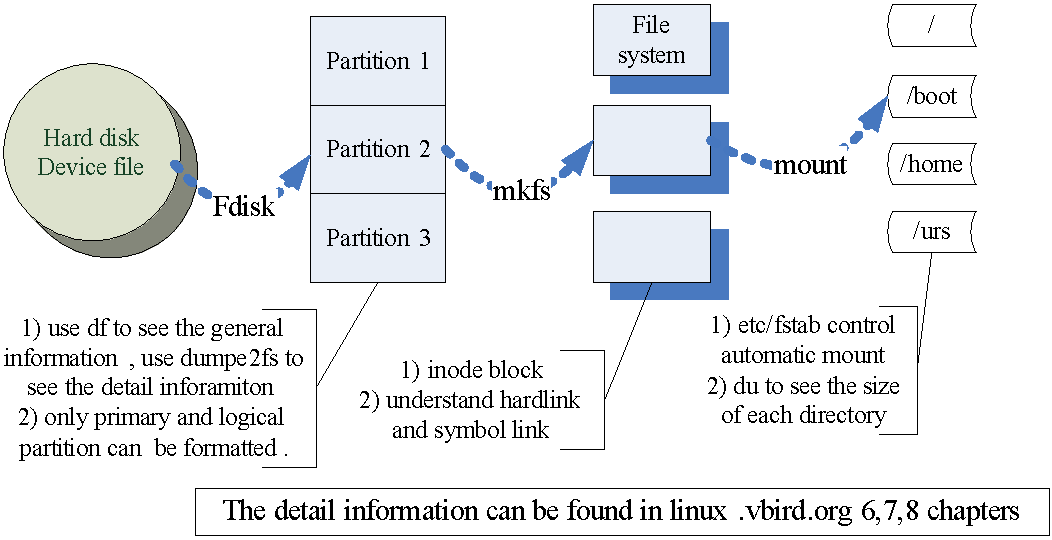
\includegraphics[scale=0.8]{pics/basic_file_system_clip}
	\\ 
   A good tool software in linux system is GParted, which  is used for creating, deleting, resizing, moving, checking, and copying disk partitions and their file systems.  You also can use df command to check your system \textbf{partitions}. You can create 1) partitions by GParted 2) mkdir a dir 3) then mount them by adding below text in /etc/fstab file.    \\   
   \verb=/dev/sda3 /home/yan/llvm ext4 defaults 0 0=
   
   \textbf{/etc, /bin, /dev, /lib and /sbin can NOT be put in different partition with root /. }  \\

\subsubsection{permission or file mode}
\begin{itemize}
      \item \linuxcommand{ls -al} will list all the files ownership and permission. Basiclly, all the system support \linuxcommand{ll} command directly. 
  \item There are three different groups: owner, Group, and Other. In each group,  there are three
      different permissions: r, w, x;
  \item for File and Dir, "rwx" has different meaning. x for Dir means you can come into
      this dir.  For a Dir, if you only have r permission, you only can \linuxcommand{ls -l
      Dir}, You can't cp a file from it unless you have x permission. So x permission is
      very important for a Dir
      \item \linuxcommand{chown chgrp} are very useful when you copy files to other
          peoples. \linuxcommand{chgrp -R grpName dirName}, you must make sure grpName in /etc/group file. or it will report error.  \linuxcommand{chown} command need to make sure owner name in /etc/passwd file. 
          \item When you need to use chgrp or chown? When you copy a file to other people. 
       \item \linuxcommand{chmod} command follow[ugoa][+-=][rwx], for example,
           \linuxcommand{chmod u+x file}  or \linuxcommand{chmod go=r file}. there are four letters:
		   u(owner), g(group), o(other) and a(all).\textbf{u represent owner, You need to remember that specially}
\end{itemize}


\subsubsection{commands about File}
\begin{itemize}
\item \linuxcommand{du -h} command displays the sizes in kilobytes of all files in the specified directory.  df command displays the amount of unused space left in your disk system. 
\item \linuxcommand{pwd} return where you are
\item \linuxcommand{cd -} will return the previous path
\item \linuxcommand{diff a.cpp b.cpp} will show line-by-line differences. 
\item In GUI, you can drag a file into terminal. 
\item when you run a command, sometimes you need to \linuxcommand{./a.out}. "./"
    means current directory.
    \item When you use cp, you need pay attention to -a options, it related to maintains
        permission and owners.
        \item You can use \linuxcommand{od} to see the binary file, It reminds me the UltraEdit
        
        \item \linuxcommand{rmdir} only can be used to delete an empty dir. You can use
            rm -r to delete a directory with files in it.
            \item \linuxcommand{tail, head, cat ,tac, less } less will stop, to ask you to
                continue. Maybe less is better than cat \\
                I often copy-and-paste text from the web into a file like this (command prompt shown):
                \begin{verbatim}
                $ cat > filename
                <Cmd-V>
                <Ctrl-D>
                \end{verbatim}
            \item \linuxcommand{which -a command} will help you find command's name
                and in all \$PATH directory.  \linuxcommand{type} can tell you if a command is
                bash build in command. such as cd command.  They are used to know more about your commands
             \item \linuxcommand{file} is to determined the kind of all files.( executable, text, or data file).  
                
             \item \linuxcommand{locate} can help you find a file very quickly, because it just search in an index database.   you can use \linuxcommand{updatedb} to update this database. \linuxcommand{whereis} just look for binary(-b option) or source(-s option) files. They just used to search binary and source files. 
                 \linuxcommand{find} to perform a throughout search, usage is complex, see below.   
                 
             \item \linuxcommand{du -h | sort -h}  display all the directory sorted by size.
\end{itemize}

\subsubsection{find command}
\begin{itemize}

	  \item \linuxcommand{find . -name "tex*"} can help you find all tex* file from current directory recursively. It's a very powerful command, without -name, it will search all the files.  Don't forget double quote around tex*. It will give tex* directly to find command. if you don't do that, shell will expand it by itself. and it will not search recursively. 
	  
	  \item You can find according to \textbf{name, type ,size, owner and time. }  \\
	  	  
     \begin{enumerate}
     	  \item \linuxcommand{find ./dir -maxdepth 1 -type d -iname "man*" } -type can be b(block), c(characer special file) d(directory), p(pipe), l(symbolic link) s(socket), or f(plain file).   -iname means ignore the case of the name. 
     	  \item \linuxcommand{find !(-not) -iname "man" } use ! or(-not).  ! or(-not) means to exclude "man" 
     	  \item \linuxcommand{find -name '*.php' -o -size +20M} Default it AND, if you want to use OR, use -o.  
     	  \item \linuxcommand{find \$HOME -ctime -2 -name "*.cpp"} -ctime(-cmin) +n|-n|n: Find files that were changed more than n (+n), less than n (-n), or exactly n days ago. cmin is minutes. About ctime and mtime, can be seen previous explanation. 
     	  \item \linuxcommand{find . -size -50M -size +20M}  c:bytes, k:kbyte, M:Mbyte G: b:512-byte blocks. Find all files smaller than 50M and bigger than 20M. 

     	  \item \linuxcommand{find . -user yan -group UH -perm 644}, see -user, -group and -perm. 
     	  
		  \item for symbolic link, you can see -H, -P, -L options in find command man page. default is -P, means that Never follow symbolic links.
\item \linuxcommand{ find . *.txt} and \linuxcommand{find . "*.txt"} are different. In the first example, shell will receive *.a and expand it to a.txt b.txt c.txt.... In the second example, find command receive *.a.  So the first find command, If in your current directory, there is a.txt. find will not look all *.txt recursively.  
\item In the previous example, you also can use \linuxcommand{find . $\backslash$*.txt}. Use $\backslash$ to escape the original means. 

  \end{enumerate}
     
     	\item 
 \end{itemize}


\subsection{User}
\begin{itemize}
\item \linuxcommand{cat /ect/passwd} will tell you all the users and which shell they are using.
 \item Don't log in root, you can use \linuxcommand{sudo } follow your command
\item \linuxcommand{whoami} tell you account informaiton.
\end{itemize}

\subsection{Internet}
	\begin{itemize}
	\item You can google "where is my IP address'' to get you external IP, or use \linuxcommand{ipconfig} to know your internal IP. \linuxcommand{host} can know IP or host name from each other. Another Interesting tool is \linuxcommand{netstat} can tell you what connections are there in your computer. and \linuxcommand{traceroute} can trace the path in connection. They are some useful Internet connection tool.
	\end{itemize}

	
\subsection{Applications}
	\begin{itemize}
	\item There are two kinds of clips, one is local clip, you only can switch data within this application, such as use Ctrl+C in kile, you only can paste in kile. if you want to paste sth to other application, you should use shift+mouse selection and copy to xclip. middle button can paset it. In Emacs, Alt+W will copy content to global clip.
	\item You just try xclip in shell to see if it's installed. if it's not installed, you can use \linuxcommand{sudo apt-get install xclip}. If you use Mac, in VMware fusion, you need to configure the Linux mouse setting.  default is command+primaryButton to simulate middle button.  xclip is very useful in linux, it support copy from a vim and paste to another vim.  
	\item There are two kinds of installing method in linux, one is install from source code, The other is install binary package.
    \item If you install from source code, you need to download tarball, then read
        INSTALL or README(option), then run config to produce makefile, last run make
        and make install.
         \begin{verbatim}
	./configure --prefix="/home/yan/app" --build=x86_64-unknown-linux-gun 
	make 2>&1 | tee make.log
	make install 
    \end{verbatim}
     \item As root, you should put install a application under /usr/local. If you don't have
         su privilege, use \linuxcommand{config PREFIX=\$home/myAPP}.  It will compile
         source first, when you make install. It will copy some files to ~/myAPP/bin or
         ~/myApp/share.
     \item./Configure use Makefile.in to produce Makefile. They are a set of automatic
         tools. You can see them in c++ web directory, but they are a little complicated,
         Kdevelop also use them.  Just know them.  Below is an example to install Perl.
	 \item install some perl programe, If you want to install in your own directory, you can add PREFIX. That will assure you have permission on it \\
  	 perl Makefile.PL
    \begin{verbatim}
    perl Makefile.PL PREFIX=\storage\yzhao
    make
    make test
    make install
    \end{verbatim}
	\item Before you install installing package, you can use \linuxcommand{md5sum} or \linuxcommand{sha1sum} on the package to get fingerprint, then compare your fingerprint with official one on the
website to check the files validation.

    \item To make less show Chinese, \linuxcommand{export LESS=-isMrf} I don't know
        what it means?

    \item There are two main binary installing method RPM+YUM(online update) and
        dpkg+APT(apt-get) . centOS uses the first, and Ubuntu uses the second. Detail
        can be found in Vbird linux book.

    \item usually, virtual box think right Ctrl as default host key, it's not convinent in linux,
        because most of move command need right Ctrl, so you need change it.
	In window, run VBoxManage.exe setextradata global GUI/Input/HostKey 165 can change it to right Alt. Here, I need to explian, the 165, it's virtual keycode defined by
	microsoft. you can find detail in google. Now I change it to Win\_L, value is 91.
	
\item There are AltGr key to input multi-language character, but I don't need it by now,
    according to my laptop layout, I need to change it to Alt, so I
	can use move command shortcut. and define win\_menu to Ctrl. I finish it as follow: \\
	1) use \linuxcommand{xev} get keycode, AltGr is 108 and win\_menu is 135 \\
	2) create your own .Xmodmap and write keycode 108 = Alt\_L\\
	3) in .bashrc, add some statements\\
	xmodmap -e "add Contrlo = Menu'' (this statement is very important)\\
	xmodmap -e "keycode 133 = Control\_R''\\
		
	\end{itemize}


\subsection{processes}
\begin{itemize}
 \item CTRL-C aborts the app, CTRL-Z suspend app and put it to backgroud, CTRL-D is EOF. 
 \item \linuxcommand{ps -l} and \linuxcommand{ps aux} are two common processes check command. ps aux will product a lot content, so we often use \linuxcommand{ps aux | grep yanzhao}. In status column, S is sleep, T is stop, and R is run. 
 \item \linuxcommand{./hello \&} will put hello to background. another useful commands are \linuxcommand{fg bg, job}. \textbf{They just belongs to this bash}. You can use ONE bash shell to do multi tasks
 
 \item View all the background jobs using jobs command,  If you have multiple background ground jobs, and would want to bring a certain job to the foreground,  \linuxcommand{fg \%2} will bring the job\#2 and \linuxcommand{kill \%2} will kill it.  
 
 \item \linuxcommand{nice commandname \&} means that you run command friendly with other(not occupy all resources) and run it at background. Skuld may be a UNIX server!
	
 \item \linuxcommand{htop} will show processes dynamicly.
 \item \linuxcommand{kill PIDnumber} will kill processes with PIDnumber
 
 \item \linuxcommand{ps -f --forest} will show all the processes in hierarchy.  Just like pstree
 \item I launch a background process, either by appending "\&" to the command line or by stopping it with CTRL-Z and resuming it in background with "bg". Then I log out.
We were quite sure it should have been killed by a SIGHUP, but this didn't happen; upon logging in again, the process was happily running and pstree showed it was "adopted" by init. But then, if it is, what's the nohup command's purpose? Below is answer: For BASH, this depends on the huponexit shell option, which can be viewed and/or set using the built-in shopt command.
\end{itemize}


\section{shell}
\subsubsection{wild character and quote}
\begin{itemize}
\item single quotes preserves the literal value of each character.  Double quotes preserves the literal value of all characters within the quotes, with the exception of '\$', '`', '$\backslash$', and, when history expansion is enabled, '!'. 
\begin{verbatim}
echo '$PATH 'pwd' '
echo "$PATH 'pwd' \$PATH"
\end{verbatim}
\end{itemize}

\subsection{Environment variable}
\begin{itemize}
			
\item When bash is invoked as an interactive login shell, or as a non-interactive shell with the --login option, it first reads and executes commands from the file /etc/profile, if that file exists. Then/etc/profile.d/*.sh. Then it looks for ~/.bash\_profile,  ~/.bash\_login, and ~/.profile, in that order, and reads and executes commands from the first one that exists and is readable. The --noprofile option may be used when the shell is started to inhibit this behavior.
		

\item When an interactive shell that is not a login shell is started, bash reads and executes commands from  /etc/bash.bashrc and ~/.bashrc, if these files exist. This may be inhibited by using the --norc option. The --rcfile file option will force bash to read and execute commands from file instead of /etc/bash.bashrc and  ~/.bashrc.	

\item echo \$0 will show "bash", it's not login shell. if it shows "-bash", it is login shell.  
	
	\item Why we need variable, just like macro in C language. With varaible, we can config and customize an application outside. And we can customize a varaible to affect a lot of applications. such as \$PATH
	\item set: \linuxcommand{YanVar=123} unset: \linuxcommand{unset YanVar} check: \linuxcommand{echo \$YanVar}
	\item There are two kinds of variables: environment and user defined.
	\item \linuxcommand{env} shows all the environment variable. such as \$HOME,  \$PATH, \$LANG \$EDITOR which can specify you default editor in your system.
	\item \linuxcommand{set} list all the local environment variables and user defined varaible , that is more than env command. For example, the \$PS1.  \linuxcommand{unset} to delete an environment variable

	\item \linuxcommand{getconf} can get some system variable, such as \linuxcommand{getconf ARG\_MAX}, you can use xargs -n 50 to make command satisfy the ARG\_MAX
	
	\item In mint, maybe in your home directory, there is no .bashrc file, so you need to create one and add export PATH=\$PATH:/home/yan/openuh-install/bin  then exit the current terminal and restart a new one. Then use echo \$PATH to see if the directory has been added.
	
	\item you should create your own bin folder under your own directory. And save your own script into it.
	Echo \$PATH will show your path setting. You can export PATH=\$PATH:/storage/yzhao/bin (add path in the end.)
	to add a new directory. Linux use : but windows use ; why windows use different?

	
	\item \linuxcommand{export DEPART=Sale} and \linuxcommand{DEPART=Sale ; export DEPART} they means the same. If the export statement in a script file,
	you must use \linuxcommand{Source a.sh} or \linuxcommand{. a.sh} to run the script file, then It will affect the continuous processing. source means that this command only run in current bash, it doesn't run in a child shell.
	
	\item Every time when you open a new terminal, It will read .bashrc or .rshrcIt depends on what shell you are using, that is why you need to use \linuxcommand{echo \$0} to know which shell you are using. It will use export(bash) or setenv(csh) to load all envoriment variable. 
			

	\item If you alread in termial, you can use export or setenv command to add envoriment varaible. if these commands are in a sh file, you have to use \linuxcommand{source a.sh} to run. because, if no source command, it will open a child terminal, so after a.sh finish, child terminal will disappear, and all the environment varaible you just set in the child terminal will disappear too. 

	\item \linuxcommand{setenv} is csh command, in bash, you can use \linuxcommand{export} directly.
			

\end{itemize}
	
\subsubsection{pipe}
\begin{itemize}
  \item pipe command can be called "filter", It will accept input fomr STDIN, perform
      opersations, then send it to STDOUT. Such as grep, uniq, sort, fmt, pr, head, cut,
      tee, tr, join, paste, expand, split, tr, awk, sed, less
  \item You cann't judge if a command is filter by running it. cat will hang up to wait for
      you from STDIN, but less will show error message.
  \item xargs is also a filter, you can use this way \linuxcommand{find . -name "*.c" |
      xargs rm -rf } a.c and b.c will be rm command arguments.
  \item Sometimes, a command need a file name as input or output, but you don't want
      to give a filename, It usually used in pipe commands, such as \linuxcommand{gzip
      -dc a.tar.gz  | tar -xvf  - }. It just like \linuxcommand{gzip -dc a.tar.gz  | tar -xvf  /dev/stdin}

\end{itemize}

\subsection{shell script}
\subsubsection{Basic}
\begin{itemize}
\item The first line of script is \verb=#!/bin/bash=.  This is a special clue given to the shell indicating what program is used to interpret the script. Other scripting languages such as perl, awk, tcl, Tk, and python can also use this mechanism.
\item After you finished script file, use \linuxcommand{chmod +x your-script-name}
\item echo -e "aaa$\backslash$nbbb" will output two lines
\item \linuxcommand{!!} run the previous command, \linuxcommand{!\$} is the previous
    argument. \linuxcommand{\$?} is the last bash command result, If it's 0, means that everything is OK. Detail can be found in google "Become a Command Line Ninja With
    These Time-Saving Shortcuts''
\item \linuxcommand{command1;command2}.   To run two command with one command line.  \\ 
\linuxcommand{command1 \&\& command2} command2 is executed if, and only if, command1 returns an exit status of zero.  \\
\linuxcommand{command1 || command2} command2 is executed if and only if command1 returns a non-zero exit status.
\end{itemize}

\subsubsection{Variable} 

\begin{itemize}
\item \$0 is script name, and \$1, \$2.. are arguments to the scripts. 
\item print the contains of variable (HOME) and not the HOME. You must use \$ followed by variable name to print variables cotaines. \verb= echo $HOME= print the variable contents. and \verb=echo HOME= just print "HOME" string. It's a little confused for a C programmer, but you need to be used to it. 
 \item In most cases, \$var and \${var} are the same: 
\item The braces are only needed to resolve ambiguity in expressions: such as echo \$\{var\}bar
\item \$(command) is `command 

\end{itemize}



\subsection{useful command}
\subsubsection{grep command}
\begin{itemize}
\item \linuxcommand{grep -r -w -i 'match' file1 file2} put files name in the end. That is basic pattern. 
\item \linuxcommand{grep --include=\*.{c,h} -rnw  -e "pattern" '/path/to/somewhere/'} -r or -R is recursive, -n is line number and -w stands match the whole word. -l (letter L) can be added to have just the file name. This will only search through the files which have .c or .h extensions. Similarly a sample use of --exclude: 
\item -c will only print  match number, -C3 will print context 3 line information . Other usage can be see in grep --help. 
\item Since you usually type regular expressions within shell commands, it is good practice to enclose the regular expression in single quotes (') to stop the shell from expanding it. 
\item grep support regex, You need to use -E option to support extended regex. \linuxcommand{grep -E 'abc{1,2}d' file}.  that's very power feature. Here, I just list a few basic usage. 
\item basic regex syntax:

 \begin{tabular}{|p{0.3\textwidth}|p{0.3\textwidth}|p{0.3\textwidth}|}
\hline 
sytax 	& example & 	description \\

\hline 
\^{} (Caret)	& '\^{}smug'  & 	'smug' at the start of a line \\
\hline 
\$ &  'smug\$' & 	match expression at the end of a line\\
\hline 
$\backslash$ (Back Slash)&   '123$\backslash$\$'  Just looke for '123\$' in file. &	turn off the special meaning of the next character, as in \^{} and \$ \{.   \\
\hline 
[ ] (Brackets)	&'[0-9][0-9]' pairs of numeric digits &	match any one of the enclosed characters,  Use Hyphen "-" for a range, as in [0-9].  [\^{} ] means excludes\\
\hline 
. (Period) & '\^{}.\$' lines with exactly one character  &	match a single character of any value, except end of line. \\
\hline 
* (Asterisk), ? , + &  &	match zero or more*,  + (pluse) is one or more,   ?(question mark) is zero or one occurrence.   \\
\hline 
\{x,y\}, 	\{x\}	\{x,\} & &	\{x,y\}match x to y occurrences of the preceding;  or \{x\} x occurrence; or  \{x,\} x or more occurrences. \\
\hline 

\end{tabular}

\item '[abc]+',  '(abc)+' and 'abc+' are different.  (abc) means it's a group, and should be considered as whole. abc+ means that + just used on letter c, So it will match ab or abc.  

\item '<.+>' will math "<car>...</car>". Default it use greedy match. If you want to use lazy match, use '<.+?>'. When you use '<.+?>'.  You should use \linuxcommand{grep -P '<.+?>'} -P means that use perl language standard. 

\item Usally, grep just match one line. If you want match multilines. You can use \linuxcommand{grep -Pnzo 'BLOCK($\backslash$n|.)*?END\_BLOCK }.  Pay attention it use lazy match method. and . doesn't means newline, you need to use '($\backslash$n|.)*?'


\end{itemize}


\subsection{VNC server}
\begin{itemize}
 \item It can help you to get remote linux desktop, It's very helpful for a windows programmer to use GUI in the linux host.
 \item vncserver -help will list all the command optoins.
 \item  You need to install VNC server in the linux with su priviliage, then run vncserver on the linux machine. Last on you windows machine, you can use putty and vncviewer to access the remote desk top. Detail can be googled, there are some reference pages available.
\end{itemize}


\chapter{Vim}
\section{basic}

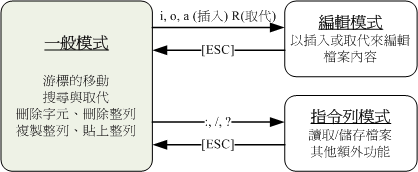
\includegraphics[scale=0.6]{pics/vi-mode} \\

\subsection{vim and terminal}
\begin{itemize}
    \item When you use solarized plug in(theme), you have to change the
        terminal. For some new version gnome terminal, you can see
        terminal->preferences->profiles->color tab, there is solarized dark
        option in "text and backgroud color", and solarized option in "build in scheme in palette", just select it.
    \item When you have old terminal, There are two options, for some old gnome
        terminal, there are no import color option, you can download
        Anthony25/gnome-terminal-colors-solarized in a temp directory, and then
        come to this directory and run .install. You need to first add an solarized profile, then the application will ask if which profile you like to overwrite, select solarized profile, you can keep you original default unmodified. Then you can select your solarized profile, the color will be set properly. 

\item If some keyword highlight background color is not correct, you need add \verb!set t_Co=16! to your .vimrc. 
    \item For mac, you can download
        tomislav/osx-terminal.app-colors-solarized(I haven't tried it yet). Or
        you can download git:altercation/solarized. there is directory \verb!osx-terminal.app-colors-solarized/!, you can import *.termnial file in
        your mac terminal preference color. That is all.
\end{itemize}

\subsection{Basic knowledge}

\begin{itemize}
	
\item Use Vim to launch vi, Vim is better than vi, previous figure is very important, you should click i to get insert mode. Then --insert will show on the bottom. If no --insert, that is common mode. All the edit command(copy and paste) should be done under common mode. 

\item \linuxcommand{sudo apt-get install vim-gnome}, then use \linuxcommand{vim -g} will support mouse.  with mouse, you can click a position to move there. you also can drag mouse to select a block of text. It's easier to use it. 

\item :h s will give you detail information about each command. 

\item \linuxcommand{vim -v} will open read-only files, \verb!zz! in normal mode  will write and quite vim.

\item .vimrc and .gvimrc are two important configure files, gvim  will read .vimrc first, and then read .gvimrc files.  You can use \verb=if has('gui_running')= to just configure for gvim, not vim in terminal. 

\item If you run vim in a terminal windows, terminal windows font and size will affect vim.  If you run gvim, You can configure vim font by add to .vimrc files.  

\item gvim's color is sharper than vim in terminal.  Maybe it use more colors than terminal.  

\item \linuxcommand{vim -u NONE} will laungh vim without laod .vimrc. It will
    help you if you have some troubles in your .vimrc file or you want to do
    some experiments. 
\end{itemize}

%最好用vim命令启动vi, 这个功能更强大一些。上面这个图非常重要,你需要经常点击i,如果进入插入模式,底部会出现--insert--的字样,
%否则就是一般模式了。所有的编辑控制(拷贝粘贴等)命令都需要回到一般模式(通过esc来完成。)理解了三个模式, 就可以很好的使用vim了。

\section{basic command}
	\begin{itemize}
	\item move, you should be able to move in both insert mode and normal mode.
			for some simple move, you should not leave insert mode, that means you can save some time.You need to use \verb!inoremap! to map to alt key, see next item.

	\item All <A-*> need to be use \verb!inoremap <A-t> <C-o>gg! command to map to a command in normal mode. In table, I just keep <A-*>, detail mapping can be seen in my .vimrc file. 

	\item there are few rules you need to follow:
			\begin{enumerate}
					\item Don't change any command in normal mode, when you use laptop or other compouter, when your mapping doesn't work well, you can return to normal mode to use these original commands in normal mode
					\item when you mapping, you can refer the normal mode, such as <A-w> is move to next word, just like w command in normal mode
					\item try your best don't leave insert mode, so mapping the mose used command in insert mode, by now, I mapping some move and editting command in insert mode.
					\item By now, you can use Alt-char map some, and You also can use two captive lettes which do use very often in our language. such as XC XV etc. 
					\item By now, on some computers, if you map alt-(char), It doesn't work very well. Sometimes, when you press it,it will go into the normal mode. I don't have time to investigate right now. 
			\end{enumerate}


	\begin{center}
		\begin{tabular}{c|c|c}
		\hline 
        move position & insert mode & normal mode \\

		\hline
		b/e of document &  <A-f>(begin)  & 1G(or gg) , G  \\

	    \hline 
		b/m/e of screen & <C-o>... & H, M, L \\

		\hline 
		pre/next para & <C-o>... &\{ \} \\

		\hline 

		pre/next sentence & <C-o>.. & \( \) \\
		
		\hline 
		begin, end of line &<A-i>and <A-a> & (0 or \^) and (\$ or g\_)  \\
		

        \hline 
        above, next line &<A-p> and <A-o> & O and o\\

	   	\hline 		
	     next, previous word &<A-w>, <A-b>  & w, b, e\\   
		
         \hline 		
         match parenthes & <C-o>... & \%   \\
         
         \hline match next character &<A-q>, <A-z>& fx, Fx \\
         
         \hline next, previous paragraph &<C-o>... & \} or \{ \\

	   	\hline
		number+ command mode &<C-o>... &  3w  4j and 15gg  \\
        
        \hline return to mark & <A-m> <A-n> & ma, then `a. \\
        
        \hline return to previous position & <C-o>... & <C-o> \\    
      				
		\hline
        search &<C-o>...  & / and ? \\
       
\end{tabular}
h,j,k,l, w(W), e(E), b(B), \^, \$ ,fx, \(, \{, gg All these move command you can add number before them. For example, 4f, will jump to the fourth ,(comma) directly.    

 scroll command, scroll window, but cursor will stay in the same position.
		\begin{tabular}{c|c|c}
        \hline
        scroll one  page &  <A-t> and <A-y>  & ctrl+b and  ctrl+f    \\
        
        \hline 		  
        scroll one line &  <A-u> and <A-r>  & ctrl+e and ctrl+y \\
        
         \hline 		  
        move cursor to m/t/b & UU RR    & zz zt zb \\

    \end{tabular}
\end{center}
 
\item d, y, c follow motion, c go to insert mode. y keep contents, For example, d2w will delete next two words. d3j will delete next 3 lines.

\item x stay in normal mode, s go into insert mode, r need to follow a letter and stay in normal mode too.

\item 3dd and 2dw   \& support number+command means how many times you will perform this command.

\begin{center}
		\begin{tabular}{c|c|c}
		\hline
		delete & insert mode & normal mode\\

   	    \hline 
		delete previous character & backspace,<C-h> & hx(move then x)  \\
		
	
		\hline 
		delete and replace current character & <A-x> & x , s , r\{char\}  \\
	
		\hline 
		delete word to end & <A-c> &dw or cw  \\
		
		\hline 
		delete word to begin & <C-w> &db or cb  \\
		
		\hline 
		delete line to end & <A-v> & d\$ or c\$  \\
		
		\hline 
		delete line to begin & <C-u> & d\^{} or c\^{}  \\
		
		\hline 
		delete current line & <A-d> & dd cc \\


		\hline 
		u and . (ctrl+r)  & <A-e> & under and redo \\
		
		
				\end{tabular}
	\end{center}



\item move and window

\begin{center}
   
  \begin{tabular}{c|c|c}
   \hline
		move & insert mode & normal mode \\
		
\hline 
		switch window & map <C-ijkl> &  Ctrl + w\{h,j,k,l\}\\
				
		\hline 
		split window &  &  Ctrl + ws\\
		
		\hline 
		switch windows & <A-g> & Ctrl + ww\\
		
		\hline 
		close a window & map <C-c> & Ctrl + wq\\
		
		\hline
		split window vertically	& & Ctrl + wv \\
		
			\end{tabular}
	\end{center}

\item move  buffer



\begin{center}
  \begin{tabular}{c|c|c}
   \hline
		move & insert mode & normal mode \\
		
\hline 
		edit a file in a new buffer & &  :e file\\
				
		\hline 
		next, previous buffer & &  :bn :bp , <C-\^{}> \\
		
\hline 
		go to number buffer & &  :b num \\		
		
		\hline 
		delete a buffer & & :bd \\
		
		\hline 
		list all open buffers & & :ls\\
		
		\hline
		open a file in a new buffer and split window
	 & & :sp :vsp \\
		
		
			\end{tabular}
	\end{center}


    
    \item copy and paste:
    
    \begin{center}
        \begin{tabular}{c|c}
		copy & paste\\
		\hline v & begin to select\\
		y & copy\\
		d & delete\\
		p & paste \\
		yy & copy the whole line, then you can use p command  \\
		
			\end{tabular}
	\end{center}
	

		
		
		\begin{center}
		\begin{tabular}{c|c}
				
		
		\hline
		search & \\
		\hline 
		/word and ?word & find word next and previous\\
		\hline  
		n and  N & continue next and previous\\
		\hline  
		:s/s1/s2 & replace in current line\\
		\hline  
		:\%s/s1/s2/g & replace in all lines\\
		\hline
		\end{tabular}
	\end{center}


	\begin{center}
		\begin{tabular}{|p{0.25\textwidth}|p{0.75\textwidth}|}
		\hline buffer &  \\
		\hline :r file & read file to current buffer \\ 
		\hline :e file & read file to new buffer, you can't open a file in current buffer, you have to :bd first then :e a new  \\ 
		\hline :badd file  & add another buffer  \\
		\hline :buffer name or num, ctrl+\^{} & switch buffer \\ 
		\hline :bd  & delete buffer \\ 
		\hline 
		\hline windows &  \\
		\hline :sp & 2 windows open files \\
		\hline ctrl+w ctrl+w  & switch window \\
		\end{tabular}
	\end{center}
	

\end{itemize}

\subsubsection{Programmer tips}
\begin{itemize}
 	\item in .vimrc file add below for c++ programming
	\begin{verbatim}
set tabstop=3
set shiftwidth=3
set number	
	\end{verbatim}
	\item In some system, Vim looks like very ugly, I have tried vim solarized dark, It looks comfortable, you can see how to install it by google it. it seems that very easy.  In mac, you can open macvim directly.  For simple use,  I have download vim-colors-solarized-master and copy it to CD. There is README.mkd file, you can see it how to install it. it's very easy.
	 
	\item  1) ma, mark the current position; \\
	           2)gD, go to the func or variable defination, \\
	           3) `a, return back mark a. \\ 
	 \item ctrl+v will invoke visual-block, you can decrease indent of block or delete a block of comments. 
	 
	 \item 1) ctrl+v, then select block of comment source code \\
	           2) don't press esc, press I (capital i) \\
	           3) input // \\
	           4) press esc, then, all the block will be commented.  
	 \item set number; syntax on and set ai;  whenever you hit Enter to start typing on the next line, vim automatically will indent to the same amount as the previous line.
	 \item \% is useful to match parenthesis command in C language. 
	 \item you can use :make within Vim, when you hit enter, after make command, it will jump to the position of first error. My make file produces a lot of warning, so In my experiment, I didn't finish it.  
	 
\end{itemize}


\subsubsection{plug in}
\begin{itemize}
\item About vundle usage, I have add a bookmark to evernote. You just need to edit .vimrc file.  
\item When you have vundle installed, you can edit .vimrc to install others plugin. By now, I have backup my .vimrc file. When you transfer to other computer, you can use it directly. 

\item For programmer, I have installed six plugins.  vim-airline, ctrlp, tagbar,  vim-colors-solarized, YouComplete and YCM-generator me. Detail can be seen in .vimrc file.

\item vim-colors-solarized, it can be only used in vim in terminal, It only support 16 color. You need to go to  vim "color scheme test c website" (add it evernote) and select you favorite scheme. and then download it. put it in .vim/bundle/vim-colors-solarized/colors directory. Then you can modify .vimrc
\begin{verbatim}
if has('gui_running')
colorscheme blacklight
else
colorscheme solarized
endif 
\end{verbatim}

 
\item For vim-airline,  First, you need to download Powerline font(github), then ./install.sh. because vim in termial use terminal font, so you should expect it have beautiful interface. It will install font to .local/share/font. Then you should add below to .vimrc.  Put statement in if, or It will make vim in terminal a little bit ugly. 
\begin{verbatim}
if has('gui_running')
set guifont=Literation\ Mono\ Powerline\ 12   (You installed powerline font)
let g:airline_powerline_fonts = 1
endif
\end{verbatim}
\item use ctrl+p to invoke ctrlp plugin, Don't use :CtrlP command  \\ 
\begin{tabular}{|p{0.25\textwidth}|p{0.75\textwidth}|}
\hline 
ctrl+f,b  & cycle between modes \\ 
\hline 
ctrl+r & switch regex mode  \\ 
\hline 
ctrl+d & switch to filename search instead of full path \\ 
\hline 
ctrl+o, t or x & open, open file in new tab or in new split \\ 
\hline 
ctrl+z  & mark and unmark files \\ 
\hline 
\end{tabular} 

\item tagbar can show all the tag(function, varaible and macro...) in a different windows. It's better than taglist. But you need to install Exuberant ctags(Use archive manager in mint to install, It's very easy)\\
\begin{tabular}{|p{0.35\textwidth}|p{0.65\textwidth}|}
\hline 
s in tag window & change order \\ 
\hline 
space in tag window & show tag prototype  \\ 
\hline 
- and + in tag window & fold and unfold \\ 
\hline 
q in tag window & quit tag window \\ 
\hline 
\end{tabular} 

\item YoucompleteMe popup windows has bad color scheme. you can add two statments in .vimrc to change it 
\begin{verbatim}
highlight Pmenu ctermfg=Bule ctermbg=White guifg=#000000 guibg=#66cc66
highlight PmenuSel ctermfg=White ctermbg=Blue guifg=#ffffff guibg=#5cadff
\end{verbatim}

\item If you install YoucompleteMe, You don't need to install syntastic anymore, By now ,YoucompleteMe support's it's own lightwight (realtime) syntastic check. And I think that is quite enough for me.  

\item For YCM-generator, It's easy to use, jut go to .vim/bundle/YCM-Generator, then run config\_gen.py pro\_dir. The pro\_dir should includes Makefile file in it.  It will run make clean first, then dry-run make to collect all the compiler flag. It remind me the understand buildspy. 

\item  

\end{itemize}


\chapter{Developing tool}
\subsubsection{gcc}
\begin{itemize}

\item disable a few lines in the source code
\begin{verbatim}
#pragma GCC diagnostic error "-Wuninitialized"
    foo(a);         /* error is given for this one */
#pragma GCC diagnostic push
#pragma GCC diagnostic ignored "-Wuninitialized"
    foo(b);         /* no diagnostic for this one */
#pragma GCC diagnostic pop
    foo(c);         /* error is given for this one */
#pragma GCC diagnostic pop
    foo(d);         /* depends on command line options */
\end{verbatim}
 \item \linuxcommand{gcc -Wall hello.c -o hello} \op{-Wall} is an important optons, you should always use it.
  \item In general, \linuxcommand{gcc -Wall hello.c -lm -o hello} the compile opton \op{-lNAME} will attempt to link object files with a library file libNAME.a in the standard library directories.
   \item By default, gcc searches the following /usr/local/include/ and /user/include for header file. and /usr/local/lib/ and /usr/lib/ for lib files.
   \item For you own header or lib files, you can use \op{-I} and \op{-L} to  add new search directories.
   \item \linuxcommand{gcc -c hello.c} will produce object file hello.o. then you can use \linuxcommand{gcc hello.o -o hello} to produce executable file. You can these two steps just compile modified c file. It will save you a lot of compile time. \linuxcommand{gcc -c *.c}  then \linuxcommand{gcc -c a.c} last \linuxcommand{gcc *.o -o last}. A better method is to use make file.
   \item there are three environment varaible gcc to use. C\_INCLUDE\_PATH, CPLUS\_INCLUDE and LIBRARY\_PATH. you can write
   \item \linuxcommand{ldd} will tell you what lib you are using in your executable
       programme.
\begin{verbatim}
 LIBRARY_PATH=\$HOME/you_include:ohter_include
 export LIBRARY_PATH
\end{verbatim}
into .bash\_profile file.

    \item .a is static library, and .so is dynamic library. Sometimes, a lib will provide lib.a
        and lib.so at the same time. gcc will use the lib.so first. In this way, you need to use
        LD\_LIBRARY\_PATH to specify lib.so directory. Or you can use \op{-static} to tell
        gcc to use lib.a version.

    \item -DNAME defines a preprocessor macro NAME
\begin{verbatim}
 #ifdef NAME
printf ...
 #endif
\end{verbatim}

   \item About optimization, a good book is ``An Introduction to GCC-Brian\_Gough'', You can google it.

   \item In a new linux system, sometimes you need to install build-essential package,  it contains some C
       language include file and library file.

\end{itemize}



\subsubsection{IDE}
If you can access GUI, you can use code::block and kile to develop and documents. if
you login by SSH, By now, I think that best tool is Emacs, with GUD, it can debug a
program. Does Emacs support latex well? Yes, It has tex mode. \par

Windows has VS community version.  Mac has Xcode, but I didn't try it too much. 

In linux, There are many tools you can uses. The most advance tool is Eclipse. the medium tools are codelite and UltraGDB. And the simple tool is vim and gdb( gdb -tui) \\

ddd is old tool, when I use it in mint 17, It's difficult to set font.  It seems that a bug for ddd. and ddd is old tool which seems to stop developing.  \\

Then I try affinic debugger, It's a commercial software and need serial number, I look for and there is not many answers on google, Maybe it's not very popular,  and the shortcoming is white background and you cann't change color theme. so I give it up. \\

codelite is a good tool, Setting->colours and fonts->Customize->C++ , you can select Themes: Monokai\_2, and you can set font MonoSpace 11pt.  
in codelite, you need to set terminal as gnome-terminal in Setting->preferences->terminal "/usr/bin/gnome-terminal -t '\$(TITLE)' -e '\$(CMD)'"
It also use xterm as debugger output. In mint, it output ugly font.  you need to produce .Xresources file on you home directory.  I keep it on the linux software backup. 

UltraGDB is subset of Eclipse, if you just need front-end of GDB, It's the best one. You can set dark theme in Window->Preferences->General->Appearance \\

In conclusion,  front end of GDB are UltraGDB and codelite. IDE are eclipse and codelite.

\subsection{Understand}
Understand is a good tools to read a large scale software. 
\begin{itemize}
\item Don't add .h, .inc, or .inl files into understand project, It will be included by .cpp and analyze automatically. 
\item For C++, use strict option in project configuration. You can adjust c++ version in strict C++ configuration. By now, It's good to use C++11, C++14 is too new
\item In Understand ,you can use "Improve project accuracy"->"missing include files" to help you search head file automatically. 
\item For CMake file, you can use \textbf{CMake -CMAKE\_EXPORT\_COMPILE\_COMMANDS -G "Unix Makefiles"} It will produce a compile\_commands.json file. In the end, you can use \linuxcommand{und} to produce a project.und. It will includes correct configuration information.  Don't use -G "Xcode", It will not produce  compile\_commands.json file.  Detail can be seen in my EverNote bookmark. 
\item For gcc and g++ project, you can use buildspy tool in Understand, detail can be seen in my EverNote bookmark.
\item If you select "terminal" color theme, inactive code will not visiable, you can change the background color to make it visible through "Preferences"->"Editor"->"Styles"
\item When analyze a long or difficult file, "worker process killed after 2 mins", you can try "Ananlyze changed file " again. if 2 minutes is too short, you can configure it longer on this specify file by override configuration. 
\item Macro is key factor in understand project, you can define it maually, but recommended way is to use CMAKE or buildsyp or visual studio to prodce a understand project automatcilly. it will includes all the correct Macro defination and include path. 
\item You can use buildspy to build a understand project in linux, configure project to relative path "Portability" then you can move source code and understand project to Mac, and use understand in Mac to open it. the interface on Mac looks better than Linux. 

\item By now, I have two projects, one is llvm and the other is openuh.  For llvm, when you run CMake in test1 directory, It will produce some head file, when you compile use xcode or makefile, It will produce some def file. But I didn't run can compiling in test1 directory, but I have really compiled src in cmake\_release\_build directory. When i use add automaticlly search headfile, it add some files in cmake\_release\_build directory. In Understand Project Browers, you can see these three directories, in fact, test1 and cmake\_release\_build are overlapped. 

\item for LLVM and openuh, when you configure and compile the source code, It will produced some addtional files to be used in compiling in build directory. so, In the end you understand project will also include build directory in the end. 
  
\end{itemize}

\subsection{gdb}
\subsubsection{start}
\begin{itemize}
\item \linuxcommand{gcc\\g++ -g file.c\\file.cpp} you need \op{-g} to compile souce code before gdb
  \item \linuxcommand{gdb -tui} start good GUI mode
  \item \linuxcommand{gdb app} just load symbol information, then you can use run arg1 arg2.. to run this problem.
  \item \linuxcommand{help} will list classes of commands then type help follewed by class name.  or help followed by command name. 
  \item you can use another terminal to compile this file and then in you gdb to kill and run again. all the breakpoints will be keep.
  \item you can kill and run app again at any time. 
 
\end{itemize}

\subsubsection{break}
\begin{itemize}
\item \linuxcommand{break 19} or \linuxcommand{break test.c:19} or \linuxcommand{break function1}, for C++, you need to tell break function list of argument types. such as \linuxcommand{TestClass::testFunc(int)}
  \item \linuxcommand{info breakpoints} will list all the breakpoints 
  \item After you have list all the breakpoints, you will know the number of them, then you can use \linuxcommand{disable 2} to  disable the second breakpoint. {ignore 2 5} will skip the number 2 and number 5 breakpoints. 
  \item  \linuxcommand{tbreak } will just stop once, then it will be removed. 
  \item \linuxcommand{until line or functions} 
\end{itemize}


\subsubsection{step}
\begin{itemize}
\item When your program is running, send ctrl+C to stop it, and you can type continue command to restart execution.
\item list command show you current context information.
\item \linuxcommand{step} will go into the function and \linuxcommand{next} will go over the function. 
\item \linuxcommand{print} will output the variable value, and \linuxcommand{set} will set variable value. 
\item \linuxcommand{call function} and \linuxcommand{finish} will finish current function.
\item look at the contents of the current frame, you can use \linuxcommand{info frame} and \linuxcommand{info locals} and \linuxcommand{info args} 

\end{itemize}

\subsubsection{stack}
\begin{itemize}
\item \linuxcommand{backtrace} will show you the the whole stack frame, on each level, there are numbers on left.
\item \linuxcommand{frame 2} will just show that level information.
\item \linuxcommand{gdb bt} will tell you which file, which function and which line you are current in.
\end{itemize}

\subsubsection{advanced}
\begin{itemize}
\item \linuxcommand{info registers} will see all the cpu registers information.
\item disassemble main to see assembly code. 
\item for x command , you can use 4xw or 4wx, they are both ok. size modifiers include(b,h,w,g). Format include(o,x,d,u,f) and (t,a) and (c, s) and i.  
\item 
\end{itemize}

\subsection{Automaticly Build}
\subsubsection{make}

	\begin{itemize}
		\item Makefile uses compiler and shell programming tools( such as rm, cp etc ) together!
		Make command will look for makefile automatically first. So you should write you own Makefile.
		\item You also can use make –f to specify you own makefile name,
		A Makefile can be regarded as a script file.

		\item The basic part of Makefile is Target: prerequisites
                        tab comm.and
		\item To check which one has changed, if someone has change, it will call command.
That is the most important, you must remember it all the time.  And it is not difficult, isn't it?

		Comment is \#
		\item Make –p to print the default MACRO, \$@ is the names of the file to be made, and \$? Is the names of
the changed dependents.

		\item PWD :=\${shell pwd} I need to explain two thing, the first is difference between := and =, := only
expand this macro once.    PWD is macro. After you define this macro, you can use it later in you paper with
\$(PWD)!

		\item @echo can be used to output string. It also can output the variable
		\item use @ to call shell command without output command itself. Use – to tell make to ignore any error.
		\item Make all that is ok, don’t add any other element. Use default to run when you don’t give make and argument
		\item Make –p will list all the default macros
		\item A := \$(wildcard *.a)  ALL\_B :=\$(wildcard *.b)  A\_B :=\$(A:\%.a=\%.b)
		\item First, when you deal with a list of files, you use := ; second when you need aàb you need use A\_B to express this set.
		\item n order to figure out the default paths used by gcc or g++ as well as their priorities you examine the output of the following commands:
\begin{verbatim}
For C:    gcc -xc -E -v -
For C++: gcc -xc++ -E -v -
\end{verbatim}

\end{itemize}

\subsubsection{CMAKE}


\subsection{PATH and LIB}
\subsubsection{lib in linux}
\begin{itemize}
\item how to make a static lib: 1) gcc -c hello.c -o hello.o 2) ar cgs libhello.a hello.o
\item how to make a dll lib: gcc -shared -o libhello.so.1.0 hello.o . For a dll lib, you need to give major and minor version number to upgrade in the future. 
\item How an application looking for a .a lib? 1) gcc -L 2)LIBRARY\_PATH 3)/lib , /usr/lib and /usr/local/lib
\item How an application looking for a .so lib? 1) DT\_RPATH section in elf file 2)LD\_LIBRARY\_PATH 3) /etc/ld.so.cache (use ldconfig to load if you modify ld.so.cache file)  4)/lib/, /usr/lib . For example, you can use export LD\_LIBRARY\_PATH='pwd' to add current directory. 

\item LIBRARY\_PATH and LD\_LIBRARY\_PATH are different, can you tell me what difference they are. 

\item libchild.a is based on libbase.a, then you have to put -lchild in front of -lbase, or it will produce dependent problem. 

\item An application will use .so firstly, you can use \linuxcommand{gcc -Wl,-Bstatic -llibname} to force it link static lib. 
\item use \linuxcommand{ldd} can see what libs does an application depends. 
\item   \linuxcommand{nm} can tell you what functions there are in a lib: there are T,U, and W categories. 
\item \linuxcommand{ar-t} can see what .o files are included in a lib. \linuxcommand{nm -D --defined-only libname.so}
will see contents in a .so file.
\item for .so use file command, for .a use objdump -x to see if they are 32 or 64 bits. 
\end{itemize}

\begin{lstlisting}[frame=single, language=c]  % Start your code-block
int i = 0;
printf("%d",i);
\end{lstlisting}

\section{Git}

\subsection{ Basic knowledge}
\begin{itemize}
\item \emph{A basic rule:  For single person, always fetch and merge before you work,  commit and push
    after you work.  For multi persion, fetch and merge even before each commit.  Maybe other people have
    committed a new version on the remote repository. }

 \item \linuxcommand{git gc} every month to run it to optimize.

 \item In linux, you can \linuxcommand{sudo apt-get install git-all} and meld(merge tools), In windows, you can download
     msysGit and P4Merge. You need edit your .gitconfig file, showed in the next section. you can use meld or
     P4Merge to visualize conflicts in source code. In Mac, you can download git from git home website. or install Xcode, when you install Xcode, It will install git in /usr/bin. but it will not install gitk GUI tool, so you can download git from home website and install another git on /usr/local/bin directory and use gitk in this directory. 

\item The two characteristics about git is \textbf{Distribute} and \textbf{Branch}, Distribute support working
    offline, Branch can make you manage branch easily and efficiently.

\item You need to know a few important conceptions: repository, branch, commit.  paths and files. You need to
    know object of a command, such as merge command, it needs two branch. not two commits. 
   

    \item origin is repository, master is branch, HEAD is commit. A repository can have many branches, so you can use origin/master. A branch can have many commits, so you can use HEAD\^ . 
    
 \item You also need to know some low-level knowledge about git. such as tree, blob,  commit. You can use \linuxcommand{git log } to know the sha value, then use \linuxcommand{git cat-file -t (or -p) sha} to check them. 
 
 
     
    \item you can use commit --allow-empty to produce a lot commits to use as test. then use
        \linuxcommand{rebase --keep-empty } to learn how to change history. Only some practical usage can
        teach you some knowledge. For Git , Dirty Hand is very very important.
        
        \item checkout and merge are different, checkout is used to "overwrite present use history", merge is used to "combine present with history".
        
         \item When a command can be followed by <paths>, then <paths> can add a file, *.file , . (all file),  /path\_name(path\_name and recursive) and /path\_name/*(no recursive).  When you read manual, you need to know, the same command has different usage when followed by different objects. For example, when checkout followed by a branch name, followed by a commit or followed by a <paths>, detail can be seen in git book p103.  reset followed by <paths> or followed by a commit is also different, detail can be seen git book p96. 
         \item you need to understand difference between tree-ish and commit-ish. commit-ish can be used as tree-ish, but tree-ish can't be used as commit-ish. 
        
     \item For git, one important question is what you want to do? then what the basic commands can do? So you need to assemble some basic commands to finish your object. 
     
    
     
\end{itemize}


\subsubsection{ git configure}
    \begin{itemize}

  \item \linuxcommand{config -e [--global|system]}  -e is open a editor. --global means user, --system means
      /etc/.gitconfig.   If you omit options, It just produce a config file for this repository.(local)

\item It's a social website, you need to find some friends here and exchange idea. The first thing you should do is to tell other peoples who you are.  
    \begin{verbatim}
	git config --global user.name "zhaoyan"
	git config --global user.email zhaoyan.hrb@gmail.com
	\end{verbatim}

    \item In windows, .gitconfig will be saved in  \\
    C:$\backslash$Documents and Settings$\backslash$Administrator directory.
    \item \linuxcommand{git config --global core.editor notepad} (use notepad as default editor)
    \item git config --list list all the configuration
    \end{itemize}

you also can change the ~/.gitconfig file and add some content below, it will customize your own git behaves. (color and log
alias is more useful).

\begin{verbatim}
[alias]
co = checkout
ci = commit -s   ## -s means to add name and email. Important when working with others.
st = status
br = branch
oneline = log --pretty=oneline --since='2 days ago'
onelog = log -p -1
[color]
status = auto
branch = auto
ui = auto
[merge]
tool = kdiff3
[mergetool "meld"]    % or "P4Merge" in Windows
path = /usr/bin/meld
keepBackup = false
trustExitCode = false	
[diff]
tool = p4merge
[difftool "p4merge"]
path = C:/Program Files/Perforce/p4merge.exe
\end{verbatim}

 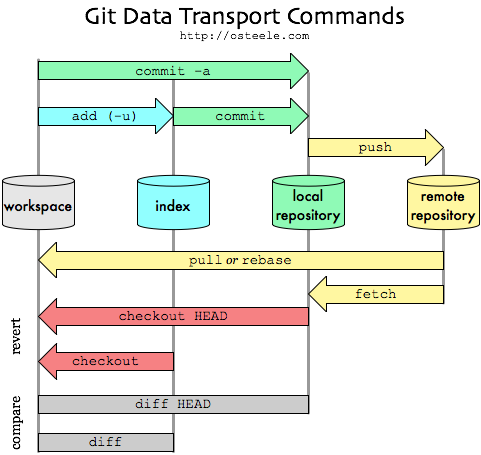
\includegraphics[scale=0.8]{pics/git-transport} \\

\subsubsection{GitHub or gitlab}
For gitHub, I have two github account:
\begin{enumerate}
	  \item zhaoyan.hrb@gmail.com  zhaoyan;
  \item yan.zhao.74@gmail.com YanZhao
\end{enumerate}
A project hello-world, Main project is on zhaoyan, then I use YanZhao account fork main project. \\
project link is : \\
git://github.com/zhaoyan/hello-world.git(read only) \\
git@github.com:zhaoyan/hello-world.git(modifiable)

\begin{itemize}
\item \linuxcommand{ssh-keygen -t rsa -C yan.zhao.74@gmail.com} \\
        	your public key has been saved in /c/Users/zhao/.ssh/id\_rsa.pub(for windows) ~/.ssh/(for Linux). Then you should paste the public key to the account in github.com. once you finish it, you can use command ssh git@github.com to test it. (github has details explanation.)\\
		You can copy id\_rsa.pub and id\_rsa to other computers. so you don't need to run ssh-keygen command any more. But when you copy id\_rsa to linux or Mac, you need \linuxcommand{chmod g-r id\_rsa} to make your private key only readable for you. Or when you push or fetch, git will refuse your request.  (ssh -v will give you verbose information. you must restart ubuntu after you move id\_rsa to ~/.ssh).


         \item{ssh -T git@github.com} will test you key setting.

\item If in your .ssh directory, you find a id\_rsa command, don't change it. You can build or modifiy config file in ~/.ssh diectory. Add something below. 1) you can use your own id\_rsa\_old name here, how to use ssh-keygen to product different name, you can see manual. 2) \textbf{Don't add Port 443 statment first, if you use ssh -T to get no response, then add Port 443, then it will work}.
		\begin{verbatim}
		Host github.com
		   Hostname ssh.github.com
		   Port 443
		   IdentityFile ~/.ssh/id_rsa_old
		\end{verbatim}

    \item Sometimes, you can't see project link, you can click the little eye(watchers) on the right upper cornor.
        pull request will show up.

\item \textbf{Don't use any Chinese in version control, If your English is not good, use
    Pinyin.}
\item In order to do anything in Git, you have to have a Git repository. This is where Git
    stores the data for the snapshots you are saving. There are two main ways to get a
    Git repository. \textbf{One way} is to simply initialize a new one from an existing
    directory, such as a new project or a project new to source control. \textbf{The
    second way} is to clone one from a public Git repository, as you would do if you
    wanted a copy or wanted to work with someone on a project.
\end{itemize}



\subsubsection{GUI}
    \begin{itemize}
    \item gitk is GUI application.
    \item gitk --all will list all the branches.
    \end{itemize}

\subsubsection{basic commands}

\begin{description}
\item[status log show] \linuxcommand{git status}  you need to use this command very often. \\

        \linuxcommand{git status -uno} will not show untracked files. \linuxcommand{git log --author=Bob} only show Bob's commit. 
         \linuxcommand{git status -s} show two columns , the first is staging, the second is working tree. if you
    modify a file,  then add. then you modify a file again. Now git status -s show MM a. guess what it means. \\
    \linuxcommand{git log} can show you all the commits history. \\
    \linuxcommand{git log --pretty=oneline} just show simply log information, easy to see.

    \begin{verbatim}
    git log -p   #show commit log and source code modification in each modification.
    git log -2  #just last two commits
    git log --after 2015-12-01  #show all commits after date
    git log --oneline  #simple informaitons
    git log --abbrev-commit --pretty=oneline #simple informaitons
    git log experiment..master #show commits on master, not on experiment
            a--b--e--f(master)
                \c--d(experiment)
    git log origin/master..HEAD #what have you push to remote?
    \end{verbatim}

    \linuxcommand{git show} to examine a single object. such as \linuxcommand{git show v1.0} and\linuxcommand{git show master:book.tex} will output source file.  It can used on commit(just like log command), or tree (just like cat-file -p). or plain blobs,(just like cat-file -p). 

\item[add commit]

When you add  a file, a blob object is produced, and .git/index(binary file) is updated to include it.  

You can use \linuxcommand{git status -uno} to hide all untraced files. You can produce a .gitignore file
in you project, it will work on present and all children directory. When you use \linuxcommand{git status}, It will
not show so many untracked files.  Example is below. edit .gitignore file \par
\begin{verbatim}
# comment
*.a   #ignore all files with .a extention
!lib.a  #but include lib.a
build/   #ignore all file in build directory
doc/*.txt  #ignore all txt files in doc/ but doc/server/arch.txt will be included.
\end{verbatim}

You should avoid using \linuxcommand{git add .} to add so many unnecessary files.  When There are a lot of files to add, \linuxcommand{add -i } is a good choice.  \linuxcommand{add -u} will only add tracked files, no dot is needed. 

Current working directory is (1),   Index file or staging is (2) and  Git local repository is (3)
      (1) -> (2) -> (3) \\
      \linuxcommand{git add} (1) -> (2) \\
      \linuxcommand{git commit} (2) -> (3) \\
      \linuxcommand{git commit -a}  (1)->(3) Don't recommend use it. \\

    \linuxcommand{git add .}   add all untracked file  \\
    \linuxcommand{git reset -- a.c}  contrary to  \linuxcommand{git add --a.c} \\
    \linuxcommand{git add -u}   it's very often used command. or It can be used in such senorita: rm *.txt, then git add -u will delete *.txt from staging. \\
    \linuxcommand{git ls-files --stage} will show all the files in stage. \\

commit command usually don't pay attention to files or directory, it just product a commit to produce a sha object(commit). \\

     \linuxcommand{git commit --amend}  don't produce new commit, just modify last commit message.\\

\item[file rename and delete]
\begin{verbatim}
rm a
git rm a // rm a can be omitted here.
git commit -m "delete file a"
git rm --ached a  //just delete a from index.

git mv a b  is three command: mv a b;   git rm a ; git add b ;
git commit -m "rename a to b"
\end{verbatim}

\item[diff]

git diff --name-only just show changed files name. so you can compare it one by one.  
git diff --name-status will show how do you changed files, add, delete or modify. \\


Before checkout or reset, you'd better to use diff command to see if there are important content to avoid
    overwrite. that is a good tip. \par

    diff -u is good command, it will show context of difference.  all the differences give by differences section.
    use @@  -1, 4  1,4 \par represent it. detail can be seen my dead wood version git book, the first chapter.

    After git fetch, you can use \linuxcommand{git diff master origin/master} to see all the modifications, then
    decide if you want to merge. fetch+merge is better than pull.
    \par

    git diff output, a stand for staging, use-symbol, b is working tree, use+symbole. You also can use
    \linuxcommand{git difftool -- file} to use meld to see the difference, it looks much better.\par

    \begin{verbatim}
git diff     ##(1) and (2)
git diff –cached   ##(2) and (3)
git diff HEAD   ##(1) and (3)

git diff tag                    ##tag and HEAD
git diff tag file               ##just compare a file (only one file name)
git diff tag1..tag2             ##two tags( you can omit two dots)
git diff SHA11..SHA12           ## two commits
git diff tag1 tag2 file or  git diff tag1:file tag2:file

#tag can be a alias of remote
git remote add xjsff git://github.com/xjsff/hello-world.git
git diff xjsff/master README  ##README and README in xjsff/master
\end{verbatim}


\item[checkout reset]

\item checkout command can checkout a file, *.file , . (all file),  /path\_name(path\_name and recursive) and
    /path\_name/*(no recursive). \par

 \item There are two different usages for checkout: with paths, it will not change HEAD. without paths, it will
     reset HEAD, HEAD will be a ref to a branch,  When It points a real commit, It will be "detached HEAD" and all
     commits after HEAD may be discards in the future. \linuxcommand{checkout commit -- paths} or \linuxcommand{checkout branch}. Don't use in\linuxcommand{git checkout commit}without paths,   such as \linuxcommand{git checkout HEAD\^ (empty) }.
    
\item checkout will overwrite work directory directory, it is not like merge, and doesn't produce conflict files. So
    be careful!

\linuxcommand{git reset HEAD} (3)->(2) \\

\linuxcommand{git checkout } no file name, like status command, show basic information. \\

\linuxcommand{git checkout . or git checkout file} (2)->(1)  \\

\linuxcommand{git checkout HEAD .}  (3)->(1) and (2) dot represents all the files \\

you can checkout a file from different locations.  \\

\linuxcommand{git checkout v1.2.3 -- filename}  tag v1.2.3 \\

\linuxcommand{git checkout stable -- filename}  stable branch \\

\linuxcommand{git checkout origin/master -- filename}  upstream master \\

\linuxcommand{git checkout HEAD -- filename}   the version from the most recent commit \\

\linuxcommand{git checkout HEAD\^ -- filename}   the version before the most recent commit \\

\linuxcommand{git checkout xxxx  --filename} xxxx is commit version number.

 Similarly, There are two different usages for reset: with paths, it will not reset commit. just like contrary operation of add \par
 
 without paths, it will reset HEAD, and all commits after reset commit will be discards( delete commits, dangerous!) \par
\begin{verbatim}
git reset <commit>-- <paths or filename>  ## (3)->(2)
git reset [--soft|hard|mixed ] <commit>
## soft just reset commit
## mixed reset commit and (3)-->(2)
## hard reset commit and (3)-->(2)-->(1)
\end{verbatim}


If you modify a file in (1), you can restore from (2) or (3), but it will overwrite (1) forever, so be careful. If you
want to keep it, you can do:
\begin{verbatim}
git add filename  ##save modify to (2)
git checkout v1.2.3 filename  ##get old version
git diff   ## compare
git checkout filename  ##restore
\end{verbatim}


\item[stash]
 Sometimes I have a situation that I am working on some feature on my own branch and suddenly someone
    comes to me and says that something really important has to be fixed or improved on the main branch.
    Usually it happens when I am in the middle of very important changes which are not ready to be committed
    for some reason. \par

Normally, I would have to save the changes (diff) into some file, switch to the main branch abandoning any
changes, apply the fix or improvement and commit it. Then I could switch back to my own branch, apply the
changes (patch) from the file and continue the work. While it is not something difficult, it can be done much
easier with Git. \par

When you use \linuxcommand{git stash}, It will run \linuxcommand{git reset --hard} automatically. so all you
work will disappear. you can use \linuxcommand{git statsh pop }to revert it.

    \begin{verbatim}
    You need to modify a bug in release version. First stash, then checkout release. coding....,commit,last git stash pop.
    git stash save “you messaage" #
    git stash list #list all stash
    git statsh pop #
    \end{verbatim}


\item[remote push pull] don't use pull, just use fetch, then merge. 
When you run \linuxcommand{git merge origin/master master}, there are three possibilities. \\
1) Working directory no modification, then fast-ward merge and working and index will be updated. \\
2) Working directory has modification, merge will fail. \\
3) Working directory has modification and commit, merge maybe ok, then working and index will be updated. merge maybe conflict, then use merge tool to resolve conflict and commit to produce a commit manually. \\

\begin{itemize}
\item origin is a alias of remote repository,  \linuxcommand{git remote add origin
    git@github.com:zhaoyan/test.git}just give a alias name, It will not real create remote repository, you need to
    log in github to create it manually.  Beside add, you can show, rename and delete a these alias. with these
    alias, you can \linuxcommand{push or fetch origion} directory, don't need to write the address of the remote
    repository.

\begin{verbatim}
git remote add paul git://github.com/paul/test.git
git remote -v
git remote show paul #show paul all the informations, including branch.
git remote rename paul pa
git remote rm pa #delete pa, because he will not contribute the system.
\end{verbatim}

\item push command is followed by a repository name and a branch name.  such as \linuxcommand{push
    origin master}. It has a lot of syntax, can be use change remote branch name and delete remote branch.

git push origin experiment \#push a branch to server\\
git push origin local:experiment \#change local branch name, and push to server.  \\
git push origin :experiment \#delete local branch ,use empty name \\
git push origin erperimental:experimental-by-yan \#give remote-tracking-branches other name,here
experimental-by-yan is remote-tracking-branches name,erperimentallocal name.
<source-name>:<destination-name> \par

\item When you push a local branch to remote, sometime it will produce non-fast-forward error. Reason is
    demonstrated by below two figures:
\begin{verbatim}
       (master)
           |
C1-->C2->C3(origin/master)
\end{verbatim}

\begin{verbatim}
             C4 (master)
           /
C1-->C2->C3(origin/master)
\end{verbatim}
In one word, from master, you can't reach origion/master, (each commit only has parent pointer).  In order to
push successfully, you have to \linuxcommand{git fetch origin} and \linuxcommand{git merge origon/master
master} firstly. Then automatically produce a new commit or manually resolve conflict and commit manually. it
will produce:
\begin{verbatim}
             C4-->C5 (master,  origin/master)
           /         /
C1-->C2->C3
\end{verbatim}

\par

If commit history look like below, you can push it successfully.
\begin{verbatim}
 (origin/master)
           |
C1-->C2->C3(master)
\end{verbatim}
\end{itemize}


\item {branch merge}

\begin{verbatim}
git branch -r  # list all the branches on the remote
git branch #list all the local branches
git branch -D b1 #delete the b1 branch
git checkout branch-name # switch to branch-name
git checkout -b new-branch master # build new new-branch from master and switch to it.
git checkout -b newbranch # build newbranch
git checkout -b newbranch origin build newbranch based on origin
git branch -m master mymaster # rename the branch
git push origin branch ,//this command will push branch to github. \\
but push branch to server isn't very meaningful, at least I think so. \\
\end{verbatim}

\begin{itemize}
  \item merge command is followed by two branches, no files name.  such as \linuxcommand{git merge
      origin/master master}

  \item merge will produce a new commit without conflict,  If there is a conflict, you need manually resolve it,
      then commit manually.

      \item When merge cann't resolve conflict, it will put working tree into a specify conditions.
      \item Three kinds of merge. 1) straight merge. 2) squash merge, 3) cherry-pick
\item \linuxcommand{git merge-base b1 b2}  found the common ancestor
\item \linuxcommand{git cherry -v master test}  in master branch, found all commits in test, but not in master.
%在master分支中,找到所有test中有但是master中没有的commit.


%主要用于将两个或两个以上的开发分支进行合并。
%主要有三种merge.第一种为straight merge. 他把一个分支的整个历史合并到另外一个分支当中去。
%还有一种就是squash 把所有的历史变成一个历史commit。 git merge --squash contact。针对于squash,
%你需要merge以后再提交。最后一种就是cherry-pick,
%git chekcout master git cherry-pick 321d76f (这是在另外一个分支提交的)。
%当然1你也可以git cherry-pick -n 321d76f. -n 告诉git先不提交,然后你就可以继续cherry-pick了。
 %然后 git commit 不用-m,这个时候一个默认的编辑器就打开了。
 %所有你pick的commit message就会自动出现在那个编辑器中。

%当merge命令自身无法解决冲突的时候,它会将工作树置于一种特殊的状态,并且给用户提供冲突信息,
%以期用户可以自己解决这些问题。当然在这个时候,未发生冲突的代码已经被git merge登记在了index file里了。
%如果你这个时候使用git diff,显示出来的只是发生冲突的代码信息。

%在你解决了冲突之前,发生冲突的文件会一直在index file中被标记出来。这个时候,如果你使用git commit提交的话,
%git会提示:filename.txt needs merge 在发生冲突的时候,如果你使用git status命令,那么会显示出发生冲突的具体信息。\\

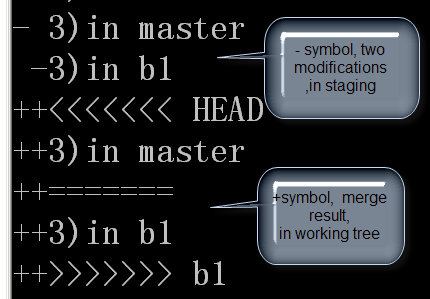
\includegraphics[scale=0.6]{pics/merge-diff} \\

after you reslove conflict 1) git add filename 2) git commit


\item If you want to revoke a branch to a status before merge \\
%如果你希望撤销一个分支到merge前的状态,那么使用如下命令:\\
git reset –hard HEAD \\–hard means working tree and index file both restore.
Or, if you've already committed the merge that you want to throw away, use this command: git reset --hard ORIG\_HEAD \\
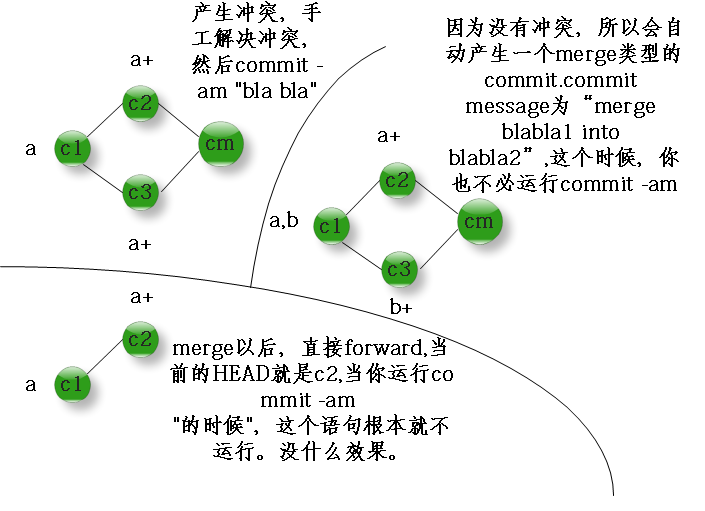
\includegraphics[scale=0.5]{pics/git-merge} \\

\end{itemize}


\end{description}

\subsection{Basic usage}

\subsubsection{clone a project from github}
\begin{enumerate}
\item  \linuxcommand{git clone git@github.com:zhaoyan/hello-worl.git}  you can copy the address from github
    website. I think that it will produce origin alias automatically.
\item modify... main.cpp
\item \linuxcommand{ git add main.cpp}  \linuxcommand{git commit  -m "modify sth..."}
\item \linuxcommand{ git log} to see if you have commit successfully.
\item \linuxcommand{git remote -v } to see what origin is.
\item \linuxcommand{git push origin master }   This command works only if you cloned from a server to which
    you have write access and if nobody has pushed in the meantime. If you and someone else clone at the
    same time and they push upstream and then you push upstream, your push will rightly be rejected. You’ll
    have to pull down their work first and incorporate it into yours before you’ll be allowed to push. (detail can be
    seen in the previous push command: produce non-fast-forwarderror.
\end{enumerate}

\subsubsection{Add a project to a git}
\begin{enumerate}
  \item \linuxcommand{cd test}, run \linuxcommand{git init}
  \item \linuxcommand{touch test.cpp}, then \linuxcommand{git add test.cpp} or \linuxcommand{git add .} dot
      means all the files. Directories are added automatically when adding files inside them. That is, directories
      never have to be added to the repository, and are not tracked on their own. You can say "git add <dir>" and
 it will add all files in there.
  \item \linuxcommand{git rm README}  you can delete a file
  \item \linuxcommand{git commit -m "first commit" } or \linuxcommand{git commit -a -m "first commit"} This is
      simple form. Combine add and commit together. Git commit -a can't add new files. If you add some news
      files, you should use \linuxcommand{git add new addfile}. then commit.

\item \linuxcommand{git log} or \linuxcommand{git status} After committing, you can use log command to
    check if it has been submitted successfully.

\item    \textbf{then, login github, create repository with name test}

\item \linuxcommand{git remote add origin git@github.com:YanZhao/test.git}
		
\item 		\linuxcommand{git remote -v }you can check remote repository
\item 		\linuxcommand{git push -u origin master} 	You can not emit origin, if you don't specify branch, default
    is master. master is default local branch, you don't need to create it explicitly. this command push local
    content
to the server.
\end{enumerate}


\subsubsection{update a project from github}
\begin{enumerate}
\item  \linuxcommand{git clone git@github.com:zhaoyan/hello-worl.git}  you can copy
    the address from github website.
\item modify... main.cpp
\item \linuxcommand{ git add main.cpp}  \linuxcommand{git commit  -m "modify sth..."}
\item \linuxcommand{git log} to see if you have commit successfully.

\item \linuxcommand{git fetch}  to get origin/master.

 \item \linuxcommand{git diff master origin/master} maybe you need to resolve conflict before you push.
\item \linuxcommand{git merge origin/master} If there are difference, you need to merge before you push, or it
    will produce non-fast-forward error.  default is local master branch, you can't write in "git merge master" to
    skip "origin/master".
\item \linuxcommand{git push origin master}

\end{enumerate}

\subsubsection{Collaborate With Applications}

\begin{description}
  \item[VS2010]  Add later

  \item[codeblock] project file is pro1.cbp, It will produce two directory bin and obj, you need to modify
      .gitignore file, add bin/ and obj/ to ignore. good suggestion.
  \item[kdevelop]
0) rm Makefile.in or .svn (if there are) \\
1) go into the src directory, and run git init \\
2) git add * and  git commit \\
3) git remote add origin git@github \\
4) git push origin master \\

0) another kdevelop, rm src\\
1) git clone git@github src\\
2) modify Makefile.am with you kdevelop project file.\\
3) in configure dialog, Configure options->linker flager -> add -L./ and add lib to the debug/src directory.\\
4) compile and run.\\

  \item[latex] Only *.tex *.bib( reference)  and /pic directory are useful are useful, You need to add them
      manually.
\end{description}

\subsubsection{single person on different computers }
On computer 1:
\begin{enumerate}
    \item \linuxcommand{git log HEAD..origin}  to check if there are differences. if true
    \item \linuxcommand{git fetch,  git merge origin/master master} ( git fetch give you more chance to
        examining it, it's better than pull)
    \item \linuxcommand{git commit -a -m " "}
    \item \linuxcommand{git push}
    \item  \linuxcommand{git log HEAD..origin }check push successfully
\end{enumerate}

On Computer 2: \\

Same operation, when you merge, it will only produce forward merge, it's relatively easy.

\subsubsection{cooperation}
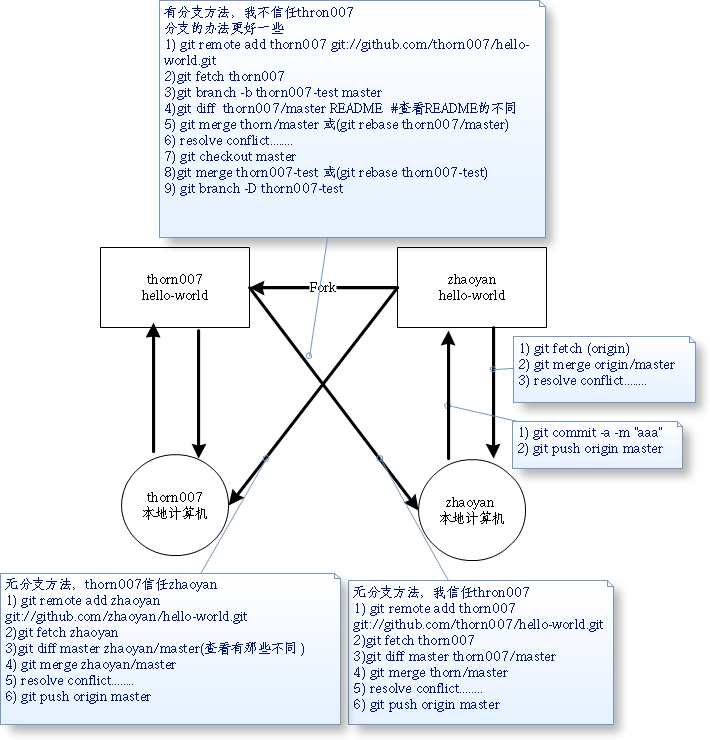
\includegraphics[scale=0.8]{pics/git-corp} \\

% \begin{verbatim}

%
% 下面我给出一个具体的例子:
% 当合作伙伴bob希望改进我(rocrocket)的工作成果,则:
% $git clone /home/rocrocket/project myrepo //此命令用于克隆我的工作到bob的myrepo目录下。请注意,此命令有可能会因为/home/rocrocket的目录权限问题而被拒绝,解决方法是chmod o+rx /home/rocrocket。
% (省略bob数小时的开发过程)…
% $git commit -a //bob提交自己的改进成果到自己的git仓库中,并口头告知我(rocrocket)他已经完成了工作。
%
% 我如果非常信任bob的开发能力:
% $ cd /home/rocrocket/project
% $ git pull /home/bob/myrepo //pull命令的意思是从远端git仓库中取出(git-fetch)修改的代码,然后合并(git-merge)到我(rocrocket)的项目中去。读者要记住一个小技巧,那就是“git pull .”命令,它和git merge的功能是一样的,以后完全可以用git pull .来代替git merge。请注意,git-pull命令有可能会因为/home/bob的目录权限问题而被拒绝,解决方法是chmod o+rx /home/bob。
%
%
% 如果我不是很信任bob的开发能力:
% $ cd /home/rocrocket/project
% $ git fetch /home/bob/myrepo master:bobworks //此命令意思是提取出bob修改的代码内容,然后放到我(rocrocket)工作目录下的bobworks分支中。之所以要放到分支中,而不是 master中,就是要我先仔仔细细看看bob的开发成果,如果我觉得满意,我再merge到master中,如果不满意,我完全可以直接git branch -D掉。
% $git whatchanged -p master..bobworks //用来查看bob都做了什么
% $git checkout master //切换到master分区
% $git merge bobworks
% $git branch -D bobworks //如果我检查了bob的工作后很不满意,就可以用-D来放弃这个分支就可以了
% 过了几天,bob如果想继续帮助我开发,他需要先同步一下我这几天的工作成果,只要在其当初clone的myrepo目录下执行git pull即可:
% #git pull //不用加任何参数,因为当初clone的时候,git已经记住了我(rocrocket)的工作目录,它会直接找到我的目录来取。
% \end{verbatim}

	if modification is small , you can use email+patch; If the modification is big, you can use fork pattern
	\begin{itemize}
    \item you can clone a exist project from other's people or on other computers,
	\item email topic()
		\begin{verbatim}
		1) git clone http://www.bitsun.com/git/gittutorcn.git
		2) edit and commit
		//method 1 (develop on master)
		$ git  fetch origin
		$ git rebase origin
		$ git for1mat path origin  ->0001-your-buddy-s-contribution.txt
		//method 2 (develop on branche, better)
		$ git checkout -b patch_mubs
		$ git checkout master
		$ git pull
		…
		$ git checkout patch_mubs
		$ git rebase master ( why I need rebase here, I want to know answer)
		
		3)email 0001-your-buddy-s-contribution.txt to vortune@gmail.com
		for vortune:
		1) git checkout -b buddy-in
		2) git am /path/to/0001-your-buddy-s-contribution.txt
		\end{verbatim}
	\end{itemize}

    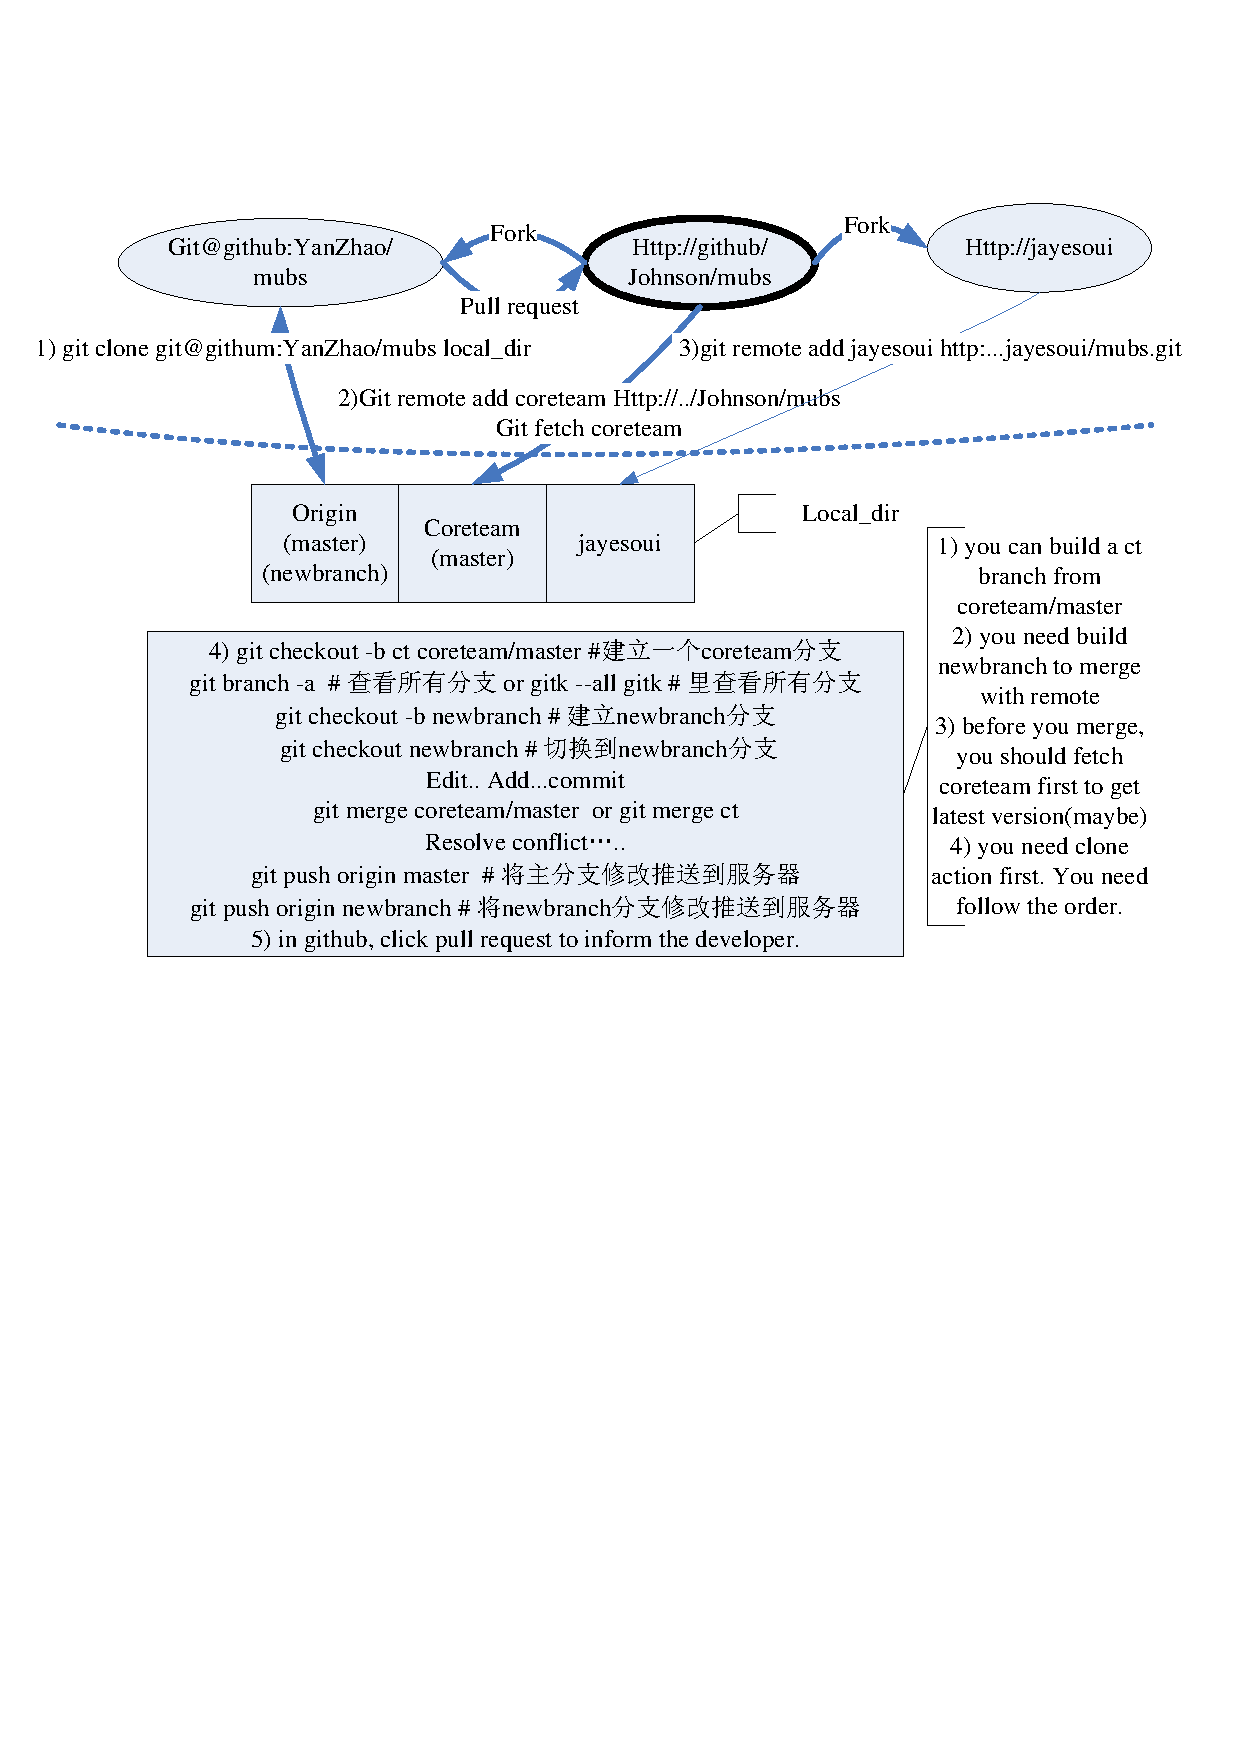
\includegraphics[scale=0.7]{pics/Visio-git_cooperate}


\subsection{ branch}

Branch can be in  two different positions. One is in the local place, you can use git branch to check them. The
other is remote-tracking branches, you can use git branch -r to check them. They have origin/albert name, origin
is not branch name, it's repository  name, and albert is branch name. \par

There are three common use branches. One is release branch which can be based on one release commit.
Usually, it used to fix some bugs in release, then you can merge back master branch. Another is feature branch,
when you add a feature, and you don't if it's good or can be finished properly, you can produce a feature branch.
The last branch is vendor branch. You don't commit on it. just keep track with upstream new version , then
merge back with you master branch.

You can not checkout remote branch, such as \linuxcommand{git checkout origin/branch1}. In order to so , you
have to create a local branch based on remote branch, such as \linuxcommand{git checkout --track -b branch1
origion/branch1}, then work on the local branch1. after you finish it. push it back. with --track, you can push or
fetch without specify remote repository name. you can omit it.


branch basic rules:\\
one branch is for (master) which is for merge, the others is for daily experiments. when you want to emerge
other's work, you need to build a branch.\\

branch is based on commit, before you make a branch, you'd better commit.\\

When you merge a branch with master, you should delete it.



\subsubsection{Cooperation based branch }
single person, center control, with branch \\
	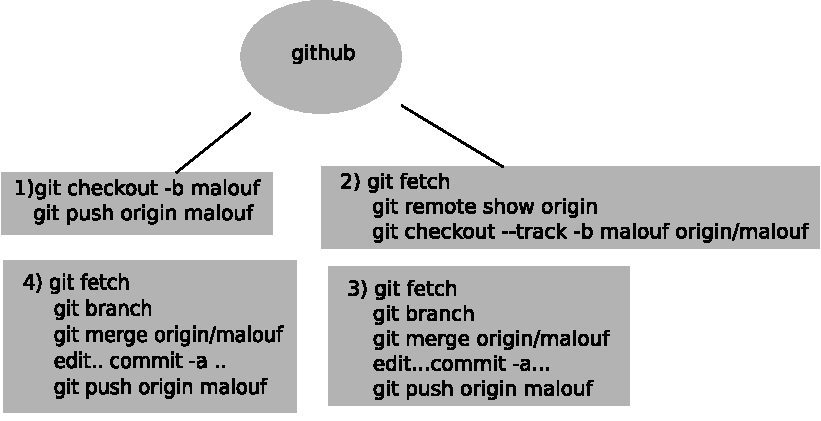
\includegraphics[scale=0.6]{pics/git_branch} \\
   	when you finish the branch, you can merge it with master.

Multi person, center control, with branch \\

   \begin{enumerate}
     \item \linuxcommand{git fetch upstream} get zhaoyan upstream the updated development process.
     \item \linuxcommand{git checkout -b test\_bla upstream/master} based zhaoyan master branch, build local
         branch test \_bla (any name is OK.)
     \item edit,  compile, \\
     git commit -am "s1" \\
     edit,  compile,  \\
     git commit -am "s2"\\
     While, upstream/master maybe changed,  a new commit t1 appear.
\begin{verbatim}
     s1--- s2
____/___t1
\end{verbatim}
\item \linuxcommand{git fetch upstream} when you want to update upstream, you have to get new commits

\item \linuxcommand{git merge upstream/master} If no conflict, produce a forward merge, if conflict, manually
    resolve and commit a new commit. \linuxcommand{git commit -am "st1"}
\begin{verbatim}
          s1--- s2
____/___t1___\st1______
\end{verbatim}

\item Or, you can use the second method: \linuxcommand{git rebase upstream/master} No conflict, produce a
    new commit. with conflict, manually resolve it, then \linuxcommand{git add conflict\_file}, then
    \linuxcommand{git rebase --continue}, not need to commit.
    \begin{verbatim}
        t1---s1--- s2
____/
\end{verbatim}

\item git push origin test\_bla

\item login github, look for you repository, checkout test\_bla, then click "request pull" button.

\item If other accept you request, you can delete test\_bla branch. \linuxcommand{git branch -D test\_bla}

\item \linuxcommand{git push origin  :test\_bla}  delete test\_bla branch in github.

\item  repeate 1-10.

   \end{enumerate}

\subsection{history}

\subsubsection{tag}
\begin{verbatim}
no space in tag name
\end{verbatim}

\subsubsection{history representation}
\begin{itemize}
\item revision \\
    \begin{verbatim}
    HEAD, FETCH_HEAD,ORIG_HEAD, MERGE_HEAD, COMMIT_EDITMSG:  #last commit
    HEAD:  #last commit。
    MERGE_HEAD:
    FETCH_HEAD:
    HEAD^: HEAD's parent, it's ORIG_HEAD

    ^ commit# first parent
    HEAD^^ : second parent
    HEAD^1:first parent
    HEAD^2:second parent

    HEAD~4:HEAD
    HEAD:README.txt
    %It represents a blob object,  sh-hash value of blob is not easy to see.
    \end{verbatim}

\item blame
    \begin{verbatim}
    git blame -L l2,l3 hello.html
    \\Who made some modification.
    \end{verbatim}

\end{itemize}



\subsubsection{history change}
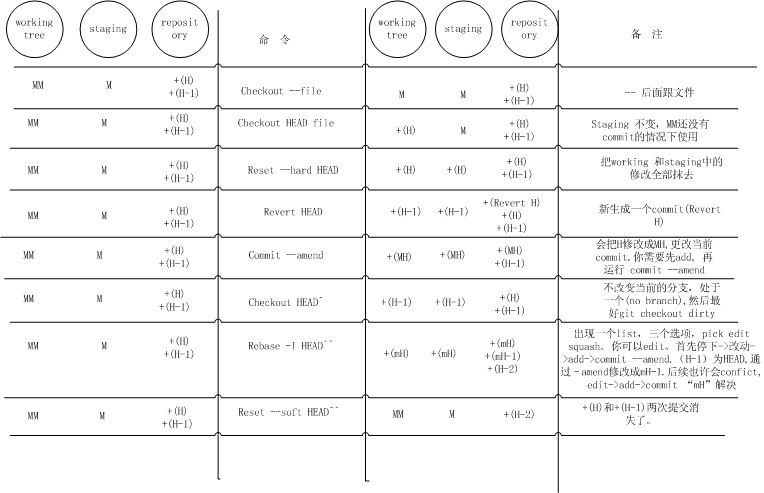
\includegraphics[scale=0.6]{pics/Git-history} \\

modify history: \\

\begin{description}
  \item[Change current lastest commit] \linuxcommand{git commit  --amend} not only change the message, but
      also the working tree contents. \verb+git commit -C HEAD^+
        will produce a new commit, but this commit is just like \verb=HEAD^ =.

  \item[delete some new commits]
   \verb=git reset --hard  HEAD^^^ = will delete \verb=HEAD^^ =  and
      \verb=HEAD^ =  and HEAD three commits
forever , It's is a dangerous  command, be careful about it.

\item[delete some old commits]
1)\linuxcommand{echo "Commit from tree of tag A | git commit-tree A\^\{tree\}}  It will produce a <SHA value> \\
2)\linuxcommand{git rebase --onto <SHA value> A master}  All the history behind of A will be deleted. \\

  \item [delete a old commit by cherry-pick ]
   1)\linuxcommand{git checkout C}, C is a tag, by now, working tree
      is C status, Here, you can't use
      \linuxcommand{reset C}, because it will put master to C,  then D, E and F will become a unreferenced
      commit, deleted by Git. If no D,E and F,
You can't use cherry-pick in the next steps.     \\
2) \linuxcommand{git cherry-pick E and F} , delete D commit ,cherry pick will produce a new commit SHA value. just like rebase.\\
3)\linuxcommand{git checkout master }  It will end Head detached status. \linuxcommand{git reset --hard HEAD@\{1\}}. Detail can be found in "Got Git". \\


  \item [delete a old commit by rebase ]
  1) \linuxcommand{git rebase --onto m2 m3 m5}, You need to know that  m3 m5 will not m3, It will produce a new commit m4 and m5,
   SHA value will be different. And from the figure, you can see that master branch is still on old m5 commit.  so you need perform next step. \\

\begin{figure}
  \centering
  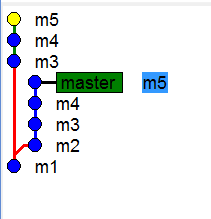
\includegraphics[scale=1.0]{pics/rebase1}
\end{figure}
  \par

  1a )\linuxcommand{git rebase --onto m2 m3 master} will keep you track master branch, after that you don't
  need to run step 2 below. It will be easy way to do that.

  2) \linuxcommand{git checkout master }  and \linuxcommand{git reset --hard HEAD@\{1\}}. After these two commands, you can see m2 has disappeared. \\
\begin{figure}
  \centering
  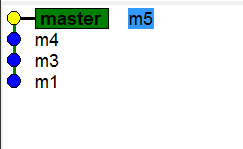
\includegraphics[scale=1.0]{pics/rebase2}
\end{figure}
  \par


  \item[combine two old commits by cherry-pick]
  1)\linuxcommand{git checkout D}, D is a tag, by now, working tree is D status,  \\
  2) \linuxcommand{git reset --soft B } ,  because HEAD is D now, go to B, --soft means working tree is still D status \\
  3)\linuxcommand{git commit -C C }  then \linuxcommand{git cherry-pick E and F}. \\
  4)\linuxcommand{git checkout master }  \linuxcommand{git reset --hard HEAD@\{1\}}. Detail can be found in "Got Git". \\

\item[combine two old commits by rebase]
  1)\linuxcommand{git checkout D}, D is a tag, by now, working tree is D status,  \\
  2) \linuxcommand{git reset --soft B } ,  because HEAD is D now, go to B, --soft means working tree is still D status \\
  3)\linuxcommand{git commit -C C }  \\
  4)\linuxcommand{git tag newbase} \\
5)\linuxcommand{git rebase --onto newbase D master}  then check \linuxcommand{git branch }to see if it's on branch master, if it's yes \\
6) \linuxcommand{git tag -d newbase } \\  Detail can be found in "Got Git". \\

\item[difference cherry pick and rebase]
1)rebase and cherry pick will change commit SHA value, so don't use
    it on any commit that you have pulled or you have
    pushed. cherry pick will not change \\
2)cherry pick should be used in change few commits, and rebase can be used to change a lot of commits at the same time.  \\


\item[delete all the commits in a merged branch]

\begin{figure}
  \centering
  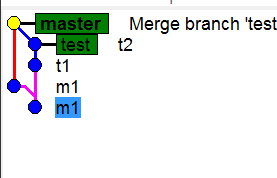
\includegraphics[scale=1.0]{pics/rebase3}
\end{figure}
  \par

1) \linuxcommand{git rebase -i -p  --keep-empty --onto 9f843b 9f843b master} -p means keep merge commit.
9f843b is m1 commit. \\

2)In git-rebase-todo file, you can see all the commits. for merge commit, you need to change it to
\linuxcommand{x git cherry-pick --allow-empty -m 1 <SHA>}, comment all the unnecessary commits. Then you
can see close this file. and rebase -i will run it according to this file. \\

3) Maybe you need to run \linuxcommand{git checkout master }  \linuxcommand{git reset --hard HEAD@\{1\}}
and \linuxcommand{git branch -D test} to make history clean.  (x options in msysGit system doesn't work, you
need to manually git cherry-pick, any way, you can see all the SHA with gitk --all command. )

\item[rebase -i] Is a powerful command, All the previous task can be finish by

\item[revert] will produce a new commit too.

\end{description}



\verb=git revert HEAD^^ = produce a new commit
 0) add a, then you don't want to put a into git.  then use git reset
-- a. if you have commit, then git rm a. It will delete a from index file,
 but in working directory still exist, then you need to commit it again. \par

1)just modify, but didn't commit \linuxcommand{git reset HEAD a.c} add but not commit. \linuxcommand{git checkout -- a.c} modify but not add. \par

2)checkout old version. \verb=git checkout HEAD^^ a.c= \par

4)return back forever \verb=git rest --hard HEAD^^= \par

5) put branch1 history into current branch.
 git rebase branch1  \par


\textbf{Never rebase branches or trees that you pulled. Only rebase local branches.
Never ever rebase a branch that you pushed, or that you pulled from another person}
\par rebase will change history, if you don't have valid reason to use it, just use merge
command.

rebase command and merge command is little different. see below:

1) in master  branch , commit few times(m1..m3), in test branch, commit few times(t1..t2). \\
 2) checkout master, then git rebase  test. \\

\begin{verbatim}
           t1-->t2
          /
m-->m1-->m2-->m3
\end{verbatim}

3) git checkout master, git rebase test, /* means that SHA value has been changed.

\begin{verbatim}
           t1-->t2-->m1*-->m2*-->m3*
          /
m-->
\end{verbatim}



%rebase的命令和merge的命令有点不太一样。一个标准的流程应该是从master创造出一个分支test,然后在test commit 几次。
%同时在master commit 几次。这个时候,进入master分支,git rebase test,


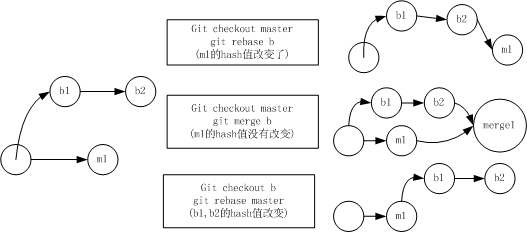
\includegraphics[scale=0.7]{pics/Git_rebase} \\

%1)如果b是一个本地的branch,如果master上没有m1那么在master 上,执行 git rebase b 和git merge b效果一样,就是增加两个新的commit。 \\

%2)如果master 上也有个更新m1。那么需要注意,如果m1只是本地的(你不是pull,同时,你还没有push)同时,你还希望保存
%b1 和 b2 两次commit。这个时候,可以使用git rebase b. (因为m1 hash值改变了,所以必须要保证本地化)。\\
%3)如果master上m1不是本地化的,那么你最好用merge。但是当你删掉b分支以后,b1,b2消失了。\\

%4)如果master上m1不是本地化的,你也可以进入b分支, 然后git rebase master,(不过你需要注意,这个时候,你还在b分支里面。)然后git checkout master , git merge b。
%相当于把b当中的b1和b2,放到了m1前面,(m1的hash没变,相当于增加了两个新的commit b1和b2. 你还需要保证b是个本地的branch)
%一句话:rebase的使用需要谨慎使用,他的本意是修改历史的作用,如果你没有很明显的理由,就直接用merge好了。\\

%rebase branch1 有三个含义,1)当前不在branch1中,2)branch1为焊接接入点,3)当前的分支commit的值改变了。

%rebase branch 与rebase master是有区别的。如果你当前在master中,并且以master为主线,那么就应该调用rebase branch。从这个角度上来说,rebase master应该用的不多。除非是上面说的第4种情况,那就是m1已经push出去,并且别人也在用。

%rebase两种常用场景,第一就是本地的分支上,两个分支出现并行情况,通过rebase branch1,可以得到相对干净的历史commit. 第二就是rebase thorn/master, 把别人的工作集成到我的master中去,(thorn/master和master都发生了commit)生成一个更干净的历史。他的基本原理和merge大致相同。






\chapter{Other Tools}



\subsection{double command}

\begin{tabular}{|c|c|}
\hline 
\textbf{key} & \textbf{action} \\ 
\hline 
ctrl+p & Place path in command combo box   \\ 
\hline 
ctrl+enter  & Append selected item to the command combo box \\ 
\hline 
shift+f2  & switch to command combo box \\ 

\hline 
ctrl shift + x & copy file Name \\ 
\hline 
ctrl shift + c & copy dir+file \\ 

\hline \hline  
ctrl+L & calculate dir size  \\ 
\hline 
ctrl+r & refresh  \\ 
\hline 
alt+enter & show property \\ 

\hline 
F9 & terminal  \\ 

\hline 
 alt+f7(Commands) & search in files(grep) \\ 
\hline 
ctrl+s  & search file name \\ 
\hline 
f2  & rename \\ 
\hline
ctrl+H  & dir history \\ 

\hline 
ctrl+command+right  & show dir right  \\ 
\hline 
ctrl+home  & home directory \\ 
\hline 
ctrl+Pageup  & parent directory  \\ 
\hline 
 
\end{tabular} 





\section{OS and phone}

\subsection{useful tips}
\begin{itemize}
\item In linux or mac, if you want to print c++ source with linenumber, you can use \\
\verb=enscript -MLetter --line-numbers -p - --word-wrap a.cpp | pstopdf -i -o ~/out.pdf=
you can use \verb=brew install enscript= to install enscript. Maybe you will see a error: you can't write /usr/local/etc.
then use \verb=sudo chown -R `whoami`:admin /usr/local/share=to give you permission. and then try brew again. 
\end{itemize}

Common used applications in each OS. in phone, I didn't install many app by now. it make you phone battery die very quickly. and I always sit in front of computer. \\

\begin{tabular}{|c|c|c|c|}
\hline & mac & windows & linux  \\
\hline diagramming & \parbox[c]{10em}{\centering OmniGraff \\ ConceptDraw}& visio & Dia   inkscape \\
\hline vector drawing & illustrator & coreldraw illustrator & ? \\
\hline edit & textmate & Ultraedit & Emacs \\
\hline doc & mactex & Ctex & livetext \\
\hline web & dreamweaver & dreamweaver & ? \\
\hline screenshot & jing snapZ pro & snagit & ? \\
\hline screencast & \parbox[c]{10em}{\centering screen flow \\ camtasia }& camtasia & Xvidcap \\
\hline download & amule or Vuze & emule & amule  \\
\hline audio editor & \parbox[c]{10em}{\centering audacity(amateur) \\ logic(profession)} & \parbox[c]{10em}{\centering gold wave(amateur)\\ adobe audition(professional)} & ? \\
\hline video editor & \parbox[c]{10em}{\centering finalcut \\  imoive(amateur)} & \parbox[c]{10em}{\centering premiere(professional) \\HuiShengHuiYing (amateur)}& ? \\
\hline
\end{tabular}
\subsection{Phone}
\begin{itemize}
  \item In my phone, weibo, webchat and web browser are three information sources.
  \item Evernote is main note tool. It can sync between phone and computer. When you have a lot note in Evernote, you can import them to latex document if you have time.
  \item In phone, you can use Everclip, on computer, you can use Evernote web clipper( in chrome browser)
  \item In Weibo or Webchat, you can repost or share it on moment. That is very easy way to keep knowledge. If this knowledge is just useful for you, you can use Everclip text, download image, or copy URL, Then use share function in your phone to save them to Evernote.
\end{itemize}
\subsection{mac}
\begin{itemize}
 \item command is window key if you use a windows keyboard.
 \item command+~ switches between documents. command+tab switches between applications.
  \item quicksiver can open and close any applications
  \item homebrew can be used to install a lot soft package from git to /usr/local/bin. It's very easy just brew install. 
  if you have older version in /usr/bin, you need to export PATH=/usr/local/bin:\$PATH. It's not very convenient. For this problem, you can down load module software, and use module load and unload, it is  environment management . 
  \begin{verbatim}
  brew install modules 
  \end{verbatim}
  
  \item 
  \begin{tabular}{|p{0.45\textwidth}|p{0.45\textwidth}|}
  \hline command +T & open a new brower \\
  \hline command+T, command + ~ & switch application or windows \\
  \hline command+shift+4 & screen snap \\
  \hline command+option+esc & force app quit(you need to command+tab switch ) \\
  \hline command+h & hide current windows \\
  \hline command+Q or W & close app or windows. \\
  \end{tabular} 
  
\end{itemize}

\subsection{win7}
\begin{itemize}
\item win+arrow key can dock windows to left,right,maximize and minimize, that is very useful
\item win+p can control project camera
\item win+1,2,3 can launch programme in task bar quickly
\item when the explore becomes slowly, you should check tool--manager add-ons to see which add-on is slow.
\item right mouse key can produce a jump list, the content of jump list will change according to the type of progamme.
\item move windows to the left side can change it to 50\% width.
\item win+L to lock the windows
\end{itemize}

\subsection{iexplore and chrome}
\begin{itemize}
\item learn to use tab to explore the internet. that is very useful, don't try to open a new page in a new windows, but in a new tab. \hotkey{ctrl+num} to navigate the tabs. and \hotkey{ctrl+click} to open a link in a new tab. \hotkey{ctrl+T} open a new tab. \hotkey{ctrl+w} to close the current tab.
\end{itemize}






\ifx \allfiles \undefined
%\end{CJK*}


\end{document}
\fi
